\part{Electromagnetism}
    \section{Electromotance and Faraday's law}
    \subsection{Sources of Steady Current}\label{sec:sources of steady current}
    Consider a conducting loop where Ohm's law, \(\vv{J} = \sigma\vv{E}\), holds.
    Then integrating along the loop with Stokes' theorem we have
    \[\oint_C\vv{J}\cdot\dd{\vv{l}} = \sigma\oint_C\vv{E}\cdot\dd{\vv{l}} = \int_S\curl\vv{E}\cdot\dd{\vv{S}}.\]
    Here \(C\) is the loop and \(S\) is the disc it encloses.
    So far we have seen that \(\curl\vv{E} = \vv{0}\) and therefore we must have that \(\vv{J} = \vv{0}\).
    However this is clearly not true so \(\curl\vv{E} = \vv{0}\) must not always be correct.
    
    Similarly
    \[\oint_C\vv{J}\cdot\dd{\vv{l}} = \sigma\oint_C\vv{E}\cdot\dd{\vv{l}} = -\sigma\oint_C\grad V\cdot\dd{\vv{l}} = -\sigma [V(2\pi) - V(0)] = 0.\]
    Again this seems to imply that \(\vv{J} = \vv{0}\).
    The only assumption made here was that \(\vv{E} = -\grad V\) which is only valid if \(\curl\vv{E} = \vv{0}\).
    So it seems that \(\vv{E} = -\grad V\) also doesn't hold all the time.
    The question is what do we have to do to fix these equations so that they apply all the time.
    
    Imagine inserting a battery between the points \(B\) and \(A\) in the loop such that it creates a potential difference of \(\Delta V\).
    If we then integrate over the whole loop but \emph{not} the battery then we have
    \[\Delta V = \emf = \int_A^B \vv{E}\cdot\dd{\vv{l}}.\]
    Here \(\emf\) is known as the \define{electromotance}, or \define{\acrfull{emf}}.
    If we assume a unit test charge then we see that
    \[\emf = \oint\vv{F}\cdot\dd{\vv{l}}.\]
    
    \subsection{Induced EMF}
    We introduce here the \define{magnetic flux},
    \[\Phi_B = \int_A\vv{B}\cdot\dd{\vv{S}} = \oint_C\curl\vv{B}\cdot\dd{\vv{l}} = \oint_C\vv{A}\cdot\dd{\vv{l}}.\]
    
    Suppose a loop of wire is placed partly in a magnetic field as shown in figure~\ref{fig:induced emf in a loop moving through a magnetic field}.
    \begin{figure}[ht]
        \centering
        \tikzsetnextfilename{induced-emf}
        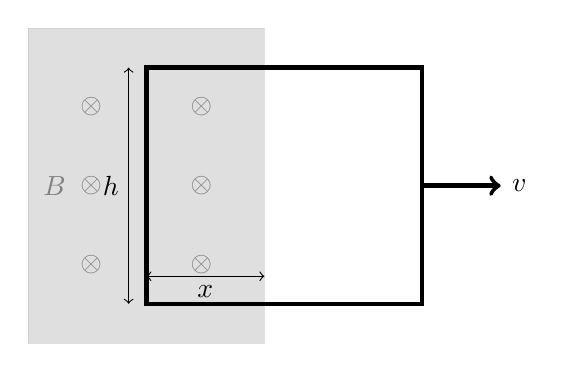
\begin{tikzpicture}
            \tikzstyle{magnetic field} = [color=lightgray, fill=lightgray, draw opacity=0.5, fill opacity=0.5]
            \tikzstyle{magnetic field label} = [color=gray]
            \tikzstyle{line} = [ultra thick]
            \draw[magnetic field] (0, 0) rectangle (3, 4);
            \foreach \x in {0.8, 2.2} {
                \foreach \y in {1, 2, 3} {
                    \node[magnetic field label] at (\x, \y) {\(\otimes\)};
                }
            }
            \node[magnetic field label, left] at (0.6, 2) {\(\vv{B}\)};
            \draw[line] (1.5, 0.5) rectangle (5, 3.5);
            \draw[line, ->] (5, 2) -- (6, 2) node[right] {\(\vv{v}\)};
            \draw[<->] (1.275, 0.5) -- (1.275, 3.5) node[midway, left] {\(h\)};
            \draw[<->] (1.5, 0.85) -- (3, 0.85) node[midway, below] {\(x\)};
        \end{tikzpicture}
        \caption{Wire loop moving through a magnetic field inducing an \gls{emf}.}
        \label{fig:induced emf in a loop moving through a magnetic field}
    \end{figure}
    The loop is dragged out of the field with a velocity \(\vv{v}\).
    The force on a charge carrier in the loop due to the magnetic field is given by
    \[\vv{F_M} = q\vv{v}\times\vv{B}.\]
    The \gls{emf} is
    \[\emf = \oint\vv{F_M}\cdot\dd{\vv{l}} = hvB.\]
    Here we have used that the force along the top and bottom parts of the loop are in opposite directions so cancel, meaning we only need to consider the contribution to the \gls{emf} of the force along the vertical section in the field.
    
    We can also calculate the magnetic flux:
    \[\Phi_B = \int\vv{B}\cdot\dd{\vv{S}} = Bhx\]
    where we define the surface normal so that the right hand rule with the current direction is satisfied.
    The flux is clearly not constant as the area of the loop that is in the field is changing:
    \[\dv{\Phi_B}{t} = \dv{t}Bhx = Bh\dv{x}{t} = -Bhx = -\emf.\]
    Note the minus sign as the area is decreasing.
    In fact the statement,
    \[\emf = -\dv{\Phi_B}{t},\]
    holds in general.
    This is called \define{Faraday's law of induction}.
    We say that this \gls{emf} is an induced \gls{emf} as it doesn't come from a normal source of \gls{emf} but rather the interaction of electric and magnetic fields.
    
    \subsection{Faraday's Law}
    Experimentally Faraday showed that altering \(\Phi_B\) by any of the following:
    \begin{enumerate}
        \item moving the surface,
        \item moving the field region,
        \item varying the field strength,
    \end{enumerate}
    produced an induced \gls{emf} in accordance with Faraday's law of induction.
    
    Note that in the last two of these the charges don't move so \(\vv{v} = 0\) meaning \(\vv{F_M} = \vv{0}\).
    Assuming that the Lorentz force law is correct there must be an induced electric field which creates a current.
    
    Faraday;s law has a differential form:
    \[\emf = -\dv{\Phi_B}{t} \implies \oint_C\vv{E}\cdot\dd{\vv{l}} = -\dv{t}\int_S\vv{B}\cdot\dd{\vv{S}}.\]
    Here \(C\) is the loop, \(S\) is the surface it encloses, and we have simply replaced \(\emf\) and \(\Phi_B\) with their definitions.
    We assume that the surface is constant so
    \[\dv{t}\int_S\vv{B}\cdot\dd{\vv{S}} = \int_S\partial_t\vv{B}\cdot\dd{\vv{S}}.\]
    We can also use Stokes' law to get
    \[\oint_C\vv{E}\cdot\dd{\vv{l}} = \int_S\curl\vv{E}\cdot\dd{\vv{S}}.\]
    Hence
    \[\int_S\curl\vv{E}\cdot\dd{\vv{S}} = -\int_S\partial_t\vv{B}\cdot\dd{\vv{S}}.\]
    Since both integrals are over the same area we must have that
    \[\curl\vv{E} = -\partial_t.\]
    We see that \(\curl\vv{E} = \vv{0}\) only holds for static magnetic fields.
    This is the full version of this law and is Maxwell's third equation.
    \[\emf = \oint_C\vv{E}\cdot\dd{\vv{l}} = -\dv{\Phi_B}{t} = -\dv{t}\int_S\vv{B}\cdot\dd{\vv{S}} \iff \curl\vv{E} = -\partial_t\vv{B}. \tag{MIII}\]
    
    \subsection{Connection to the Magnetic Vector Potential}
    If we combine \(\curl\vv{E} = -\partial_t\vv{B}\) and \(\vv{B} = \curl\vv{A}\) then we have
    \[\curl\vv{E} = -\partial_t(\curl\vv{A}) = -\curl(\partial_t\vv{A})\]
    which means
    \[\curl(\vv{E} - \partial_t\vv{A}) = \vv{0}.\]
    This means that there must exist a scalar field, \(V\), such that
    \[\vv{E} - \partial_t = -\grad V.\]
    Rearranging this we have
    \[\vv{E} = -\grad V - \partial_t\vv{A}.\]
    This is the most general way to write \(\vv{E}\) in terms of potentials, it reduces to \(\vv{E} = -\grad V\) if \(\vv{B}\) is time independent.
    We have now fixed the two equations that we showed weren't correct in section~\ref{sec:sources of steady current}.
    We see that there are two sources of the electric field:
    \begin{itemize}
        \item A stationary charge distribution, \(\rho\), which gives a contribution \(-\grad V\).
        \item A time dependent magnetic field, \(\vv{B}\), which gives a contribution \(-\partial_t\vv{A}\).
    \end{itemize}

    \subsection{Lenz's Law}
    \define{Lenz's law} is a rule of thumb that allows us to decide the sign of the flux.
    It states that the induced \gls{emf}, \(\emf\), acts in a way as to oppose the change that created it.
    For example in the case of removing a wire from a magnetic field the \gls{emf} causes a current in the wire in a direction such that the force due to the magnetic field's interaction with this current is in the opposite direction to the direction which the wire is being pulled.
    This is useful as it is often not that easy to see what the direction of the flux is and hence the direction of the induced \gls{emf} and induced current.
    
    \section{Induction}
    \subsection{Induction Examples}
    \subsubsection{AC Generator}
    A current loop, initially the \((x, z)\)-plane, with area \(A\) is placed in a uniform magnetic field, \(\vv{B}\).
    The loop is rotated at an angular velocity \(\vv{\omega} = \omega\ve{z}\).
    Since the loop is rotating the flux through the loop is time dependent:
    \[\Phi_B = \int_A\vv{B}\cdot\dd{\vv{S}} = B\cos(\omega t)\int_A\dd{S} = AB\cos(\omega t).\]
    Therefore there is an induced \gls{emf}:
    \[\emf = -\dv{\Phi_B}{t} = AB\omega\sin(\omega t).\]
    The induced current will be an AC current with a frequency \(\omega\).
    The current is \(\pi/2\) out of phase with the flux in a way that means that the peak current occurs when the flux is zero.
    
    \subsubsection{Rotating Disc of Charge}
    An insulating disc of radius \(a\) with a uniform surface charge density, \(\sigma\), is rotated around its axis.
    There is a uniform magnetic field parallel to the axis of the disc.
    The magnetic force on a charge element, \(\dd{q}\), on the disc at a radius \(r\), is
    \[\dd{\vv{F}} = \dd{q}vB\ve{\rho} = \dd{q}r\omega B\ve{\rho}.\]
    This magnetic force is equivalent to a radial electric field:
    \[\vv{E'} = \frac{1}{q}\vv{F} = r\omega B\ve{\rho}.\]
    The induced \gls{emf} between the centre and edge of the disc is then
    \[\emf = \int_{0}^a\vv{E'}\cdot\ve{\rho}\dd{\rho} = \frac{\omega Ba^2}{2}.\]
    This acts outwards to move the charge to the outside of the disc.
    If the disc were a conductor then this would actually happen.
    
    While the flux rule,
    \[\emf = -\dv{\Phi_B}{t},\]
    is still valid there is not a useful current loop to compute the flux through so it isn't of much help in this problem.
    
    \subsection{Mutual Inductance}
    Two current loops, \(C_1\) and \(C_2\) are carrying currents \(I_1\) and \(I_2\) in directions \(\dd{\vv{l_1}}\) and \(\dd{\vv{l_2}}\) respectively at positions \(\vv{r_1}\) and \(\vv{r_2}\).
    Current \(I_1\) creates a magnetic field, \(\vv{B_1}\), which passes through loop 2.
    Therefore a current is induced in loop 2.
    The induced flux in loop 2 is
    \[\Phi_2 = \int_{S_2}\vv{B_1}\cdot\dd{\vv{S_2}} = M_{21}I_1\]
    where we have used that \(\abs{\vv{B_1}}\propto I_1\) and \(M_{21}\) is just a constant of proportionality called the \define{mutual inductance}.
    If we substitute the vector potential, \(\vv{A_1}\), such that \(\vv{B_1} = \curl\vv{A_1}\), we get
    \begin{align*}
        \Phi_2 &= \int_{S_2} \vv{B_1}\cdot\dd{\vv{S_2}}\\
        &= \int_{S_2} (\curl\vv{A_1})\cdot\dd{\vv{S_2}}\\
        &= \oint_{C_2} \vv{A_1}\cdot\dd{\vv{l_1}}\\
        &= \frac{\mu_0 I_1}{4\pi} \oint_{C_2}\oint_{C_1} \frac{\dd{\vv{l_1}}\cdot\dd{\vv{l_2}}}{\abs{\vv{r_1} - \vv{r_2}}}.
    \end{align*}
    In the last step we have used the explicit solution to \gls{pe}, \(\laplacian\vv{A} = -\mu_0\vv{J}\).
    This gives us that
    \[M_{21} = \frac{\mu_0}{4\pi}\oint_{C_2}\oint_{C_1} \frac{\dd{\vv{l_1}}\cdot\dd{\vv{l_2}}}{\abs{\vv{r_1} - \vv{r_2}}}.\]
    This is called the Neumann formula.
    It isn't that useful, as it is pretty hard to calculate for arbitrary geometries, it is important to note that it is symmetric in 1 and 2, that is if we perform the equivalent calculation but completely swap the two loops we will get the same answer so
    \[M_{21} = M_{12} = M.\]
    The flux through loop 1 due to a current \(I\) in loop 2 is the same as the flux through loop 2 due to a current \(I\) in loop 1.
    
    The induced \gls{emf} in loop 2 due to current \(I_2\) is
    \[\emf_2 = -\dv{\Phi_2}{t} = -\dv{t}[MI_1] = -M\dv{I_1}{t}.\]
    We can then use Lenz's law to calculate the direction of the current noting that it must oppose any change in \(I_1\).
    
    One application of this is a spark plug in a car.
    In this loop 1 is wrapped around a core a few times and loop 2 is wrapped around the same core many many times.
    This leads to a very large value of \(M\) and so a small current in loop 1 can create a very large current in loop 2 which is large enough to spark across an air gap and ignite the fuel.
    
    \subsection{Self Inductance}
    If a loop carries a current then it generates a magnetic field.
    This magnetic field creates a flux through the loop.
    Therefore if the current is time dependent there will be an induced \gls{emf} and induced current in the loop that acts to oppose the change in the initial current.
    The \gls{emf} will be
    \[\emf = -\dv{\Phi_B}{t} = -L\dv{I}{t},\]
    where we have defined \(L\), the \define{self inductance}, to be such that \(\Phi_B = LI\).
    
    For example a solenoid of length \(\ell\) and radius \(a\) with \(n\) loops per unit length has an interior magnetic field of
    \[\vv{B} = B_z\ve{z} = \mu_0 nI\ve{z}.\]
    Each loop is approximately a closed circle of area \(A = \pi a^2\) and so the total flux through all \(n\ell\) loops is
    \[\Phi_B = \int \vv{B}\cdot\dd{\vv{S}} = An\ell B_z = \mu_0I\pi a^2n^2\ell.\]
    We can then identify the self inductance as
    \[L = \mu_0 \pi a^2n^2\ell = \mu_0n^2V_s\]
    where \(V_s = \pi a^2\ell\) is the volume of the solenoid.
    
    \subsection{Electronics}
    \textit{This section is non-examinable}
    
    We have introduced three material properties which all relate a voltage, \(\Delta V\), to the charge, \(Q\), in a different way:
    \begin{itemize}
        \item Resistance, \(R\):
        \[\Delta V \sim I \sim \dv{Q}{t}.\]
        \item Capacitance, \(C\):
        \[\Delta V\sim Q.\]
        \item Inductance, \(L\):
        \[\Delta V \sim \dv{I}{t} \sim \dv[2]{Q}{t}.\]
    \end{itemize}
    By constructing a circuit with two of these in series we can model differential equations.
    Since they are in series the voltage in all components will be the same.
    We start with a resistor and capacitor.
    From the fact that the voltages are equal we have that
    \[\dv{Q}{t} \sim Q \implies Q = Q_0e^{-\alpha t}\]
    for some constants \(Q_0\) and \(\alpha\).
    If we swap the capacitor for an inductor then we will have
    \[\dv{I}{t} \sim I \implies I = I_0e^{-\beta t}\]
    for some constants \(I_0\) and \(\beta\).
    Finally if we have a capacitor and inductor in series then
    \[\dv[2]{Q}{t} \sim Q \implies Q = Q_0'\sin(\omega t + \varphi) \implies I = Q_0'\omega\cos(\omega t + \varphi)\]
    for some constants \(Q_0'\), \(\omega\), and \(\varphi\).
    
    In the first case the charge on the capacitor decays away exponentially.
    In the second case the current that is initially induced by the inductor decays away exponentially.
    In the last case if initially we start with a charged capacitor and with no current (\(\varphi = \pi/2\)) then as the capacitor discharges a current is is induced and this charges the capacitor and we get an oscillating charge and current.
    
    \subsection{Magnetic Energy in Inductors}\label{sec:energy magnetic field}
    In electrostatics the electrostatic energy is due to the work done to create a charge distribution, done against Coulomb repulsion.
    Similarly in magnetostatics the magnetostatic energy is due to the work done to create a steady current, done against the induced \gls{emf} which opposes the creation of any current.
    
    If we try to create a current, \(\dd{I}\), in a loop in time \(\dd{t}\) we need to do work against the induced \gls{emf}, \(\emf\):
    \[\dd{U_M} = -\emf I\dd{t} = LI\dv{I}{t}\dd{t} = LI\dd{I},\]
    where \(L\) is the self inductance of the loop and we have used that
    \[-\emf = \dv{\Phi_B}{t} = \dv{t}[LI] = LI\dv{I}{t}.\]
    Integrating the energy with time we get
    \[U_M = \frac{1}{2}LI^2.\]
    Compare this to the equivalent statement in electrostatics that
    \[U_E = \frac{1}{2}\frac{Q^2}{C}.\]
    For two loops with inductances \(L_1\) and \(L_2\) carrying currents \(I_1\) and \(I_2\) with mutual inductance \(M\) then the energy becomes
    \[U_M = \frac{1}{2}L_1I_1^2 + \frac{1}{2}L_2I_2^2 + MI_1I_2.\]
    We can generalise the energy to any current arrangement:
    \begin{align*}
        U_M = \frac{1}{2}LI^2\\
        &= \frac{1}{2}\Phi_BI\\
        &= \frac{1}{2}I\oint_C \vv{A}\cdot\dd{\vv{l}}\\
        &= \frac{1}{2}\oint_C \vv{A}\cdot\vv{I}
    \end{align*}
    for a single loop.
    Notice that \(\oint_C \vv{A}\cdot\vv{I}\) is effectively a volume integral over all space of \(\vv{J}\) since this is only non-zero where there is a current, which in the case of a single loop reduces to a contour integral.
    Hence
    \[U_M = \frac{1}{2}\int\vv{A}\cdot\vv{J}\dd{V}.\]
    Where the integral is performed over all space.
    Using Amp\`ere's law we have
    \begin{align*}
        \mu_0\vv{A}\cdot\vv{J} &= \vv{A}\cdot(\curl\vv{B})\\
        &= \abs{\vv{B}}^2 - \div(\vv{A}\times\vv{B})
    \end{align*}
    where we have used the vector identity
    \begin{align*}
        \div(\vv{A}\times\vv{B}) &= \vv{B}\cdot\underbrace{(\curl\vv{A})}_{=\vv{B}} - \vv{A}\cdot(\curl\vv{B})\\
        &= \vv{B}\cdot\vv{B} - \vv{A}\cdot(\curl\vv{B})\\
        &= \abs{\vv{B}}^2 - \vv{A}\cdot(\curl\vv{B}).
    \end{align*}
    Hence the energy is
    \[U_M = \frac{1}{2}\vv{A}\cdot\vv{J}\dd{V} = \frac{1}{2\mu_0}\int\abs{\vv{B}}^2\dd{V} - \frac{1}{2\mu_0}\int\div(\vv{A}\times\vv{B})\dd{V}.\]
    We can write this last integral as a surface integral using the divergence theorem:
    \[\int\div(\vv{A}\times\vv{B})\dd{V} = \oint_S(\vv{A}\times\vv{B})\cdot\dd{\vv{S}}.\]
    If \(A\sim 1/r\) and \(B\sim 1/r^2\), as is the case for steady, finite, localised currents, then \(\abs{\vv{A}\times\vv{B}}\sim 1/r^3\).
    The surface area, \(S\sim r^2\).
    Since the volume integral is over all space the surface integral is over a boundary at infinity and so
    \[\int(\vv{A}\times\vv{B})\cdot\dd{\vv{S}} \sim \frac{1}{r^3}r^2 = \frac{1}{r}\]
    which becomes zero as \(r\to\infty\).
    Hence the energy is
    \[U_M = \frac{1}{2\mu_0}\int\abs{\vv{B}}^2\dd{V}.\]
    We can define an energy density, \(u_M\), such that
    \[u_m = \frac{\abs{\vv{B}}^2}{2\mu_0} \implies U_M = \int u_m\dd{V}.\]
    Compare this to the electrostatic case
    \[u_E = \frac{1}{2}\varepsilon\abs{\vv{E}}^2.\]
    
    \section{Displacement Current}
    \subsection{The Continuity Equation}
    The global electric charge is conserved.
    This means that the only way that the charge contained in a volume, \(V\), can change is if charge enters or leaves the volume.
    In the case that this happens there will be a current \(\vv{J}\) associated with the charge moving.
    The charge enters the volume at a rate of
    \[\pdv{Q}{t} = -\oint_S\vv{J}\cdot\dd{\vv{S}}.\]
    The minus sign accounts for the fact the surface normal, \(\dd{\vv{S}}\), points out of the volume so \(\vv{J}\cdot\dd{\vv{S}}\) is the charge leaving the volume through the surface \(\dd{\vv{S}}\), on the other hand \(\partial_t\) is the rate of increase of charge.
    Substituting in the charge density and applying the divergence theorem we have
    \[-\pdv{t}\int_{V}\rho\dd{V} = \int_V \div\vv{J}\dd{V}.\]
    Since this holds for all volumes we must have
    \[-\pdv{\rho}{t} = -\div\vv{J}.\]
    This is the \define{continuity equation}.
    It actually applies to any conserved quantity with an associated density and current.
    For example if \(\rho\) is mass density and \(\vv{J}\) is mass current which describes how mass is moving, for example it may describe fluid flow, then the continuity equation applies.
    Another important application is in quantum mechanics where \(\rho\) is the probability density and \(\vv{J}\) is a probability current which describes how the probability of different states changes with time.
    
    \subsection{Displacement Current}
    Amp\`ere's law is
    \[\curl\vv{B} = \mu_0\vv{J}.\]
    Taking the divergence of this we have
    \[\div(\curl\vv{B}) = \mu_0\div\vv{J}.\]
    The left hand side is identically zero by a vector calculus identity.
    For the right hand side we apply the continuity equation and get
    \[0 = -\mu_0\pdv{\rho}{t}.\]
    This is obviously wrong for a non-static charge distribution, \(\rho(\vv{r}, t)\), which we know can exist and would expect \(\rho\) not to be constant with time.
    Using the continuity equation we can known
    \[\div\vv{J} + \pdv{\rho}{t} = 0\]
    and so
    \[\div(\curl\vv{B}) = \mu_0(\div\vv{J} + \partial_t\rho)\]
    From Maxwell's first law we know that
    \[\rho = \varepsilon_0\div\vv{E}\]
    so
    \[\div(\curl\vv{B}) = \mu_0(\div\vv{J} + \varepsilon_0\partial_t\div\vv{E}) = \mu_0 \div(\vv{J} + \varepsilon_0\partial_t\vv{E})\]
    Since \(\div(\curl\vv{K}) = 0\) for all vector fields, \(\vv{K}\), we must have
    \[\curl\vv{B} = \mu_0(\vv{J} + \varepsilon_0\partial_t\vv{E} + \curl\vv{K}).\]
    It turns out that \(\vv{K} = \vv{0}\), this is required so that in the static case this equation reduces to \(\curl\vv{B} = \mu_0\vv{J}\).
    Therefore
    \[\curl\vv{B} = \mu_0(\vv{J} + \varepsilon_0\partial_t\vv{E}).\]
    This is the \define{Amp\`ere--Maxwell law} and is the full version of Maxwell's fourth equation with time dependent fields.
    It also has an integral form, using Stoke's theorem we have
    \[\int_S(\curl\vv{B})\cdot\dd{\vv{S}} = \oint_C \vv{B}\cdot\dd{\vv{l}}\]
    also
    \[\mu_0\int_S \vv{J}\cdot\dd{\vv{S}} + \varepsilon_0\int_S \pdv{t}\vv{E}\cdot\dd{\vv{S}} = \mu_0\int_S \vv{J}\cdot\dd{\vv{S}} + \mu_0\varepsilon_0\dv{t}\int\vv{E}\cdot\dd{\vv{S}}\]
    so
    \[\oint_C\vv{B}\cdot\dd{\vv{l}} = \mu_0\int_S \vv{J}\cdot\dd{\vv{S}} + \mu_0\varepsilon_0\dv{t}\int\vv{E}\cdot\dd{\vv{S}}\]
    What this law tells us is that magnetic fields can originate from two sources:
    \begin{itemize}
        \item Steady currents, \(\vv{J}\)
        \item Time dependent electric fields, \(\vv{E}\) (which themselves are created by time dependent charge densities or time dependent magnetic fields that change at a non-constant rate).
    \end{itemize}
    We call \(\varepsilon_0\partial_{t}\vv{E}\) the \define{displacement current} because it has dimensions of current density and creates a magnetic field.
    It is not a real current however.
    
    \subsubsection{Capacitor Paradox and Resolution}
    The capacitor paradox is another example of why Amp\`ere's law alone is not quite correct.
    The capacitor paradox is as follows.
    Consider a capacitor charging/discharging with a time dependent current, \(I(t)\),
    What is the magnetic field?
    Since the current is time dependent then so is the field.
    By Amp\`ere's law we have
    \[\oint_C\vv{B}\cdot\dd{\vv{l}} = \mu_0\int_S\vv{J}\cdot\dd{\vv{S}}.\]
    The paradox arises in the right hand side of this equation.
    If we take the surface \(S\) to cut through the wire then the right hand side is equal to \(\mu_0I(t)\).
    It is also possible to construct a surface with the same boundary in a way such that the surface goes in between the plates of the capacitor without ever intersecting any of the circuit.
    Then the right hand side of this equation is zero.
    
    We fix the supposed paradox by using the full Amp\`ere--Maxwell law.
    We known that for an ideal parallel plate capacitor the electric field is entirely constrained to be between the plates and in this volume it is normal to the plates and the field strength is
    \[E(t) = \frac{Q(t)}{\varepsilon_0 A}\]
    where \(A\) is the area of the plates.
    If we define the direction of \(\vv{E}\) to be the \(z\) direction then
    \[\varepsilon_0\partial_t\vv{E} = \frac{1}{A}\pdv{Q}{t}\ve{z} = \frac{I(t)}{A}\ve{z}.\]
    If we also choose to construct the surface so that it is parallel to the plates of the capacitor when it is between them then
    \[\mu_0\int_{S_2}(\vv{J} + \varepsilon_0\partial_t\vv{E})\cdot\dd{\vv{S}} = \frac{I(t)}{A}\int_{S_2}\dd{S} = \mu_0I(t)\]
    where we have used the fact that the field is zero outside of the capacitors so the surface integral is equivalent to an integral over the area of the capacitor.
    This is exactly the same result that we get using the other surface so we have fixed the paradox.
    \begin{figure}[ht]
        \centering
        \tikzsetnextfilename{capacitor-paradox}
        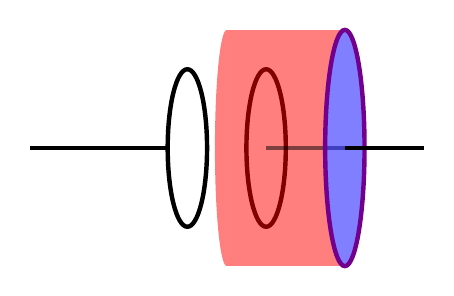
\begin{tikzpicture}
            \tikzstyle{line} = [ultra thick]
            \draw[line] (0, 0) -- (1.75, 0);
            \draw[line] (2, 0) circle[x radius=0.25cm, y radius=1cm];
            \draw[line] (3, 0) circle[x radius=0.25cm, y radius=1cm];
            \fill[color=red, opacity=0.5] (2.5, -1.5) rectangle (4, 1.5);
            \begin{scope}
                \clip (2.5, -1.5) rectangle (0, 1.5);
                \fill[color=red, opacity=0.5] (2.5, 0) circle[x radius=0.15cm, y radius=1.5cm];
            \end{scope}
            \draw[color=red, opacity=0.25] (2.5, -1.5) -- (2.5, 1.5);
            \fill[white] (4, 0) circle[x radius=0.25cm, y radius=1.5cm];
            \draw[line, opacity=0.5] (3, 0) -- (5, 0);
            \fill[color=blue, opacity=0.5] (4, 0) circle[x radius=0.25cm, y radius=1.5cm];
            \draw[color=red!45!blue, line] (4, 0) circle[x radius=0.25cm, y radius=1.5cm];
            \draw[line] (4, 0) -- (5, 0);
        \end{tikzpicture}
        \caption{The capacitor paradox. The two surfaces used in the capacitor paradox. \(S_1\) in blue goes through the wire and \(S_2\) in red goes through the gap in the capacitor. They share the boundary, \(C\), shown in purple.}
    \end{figure}
    
    \subsection{Maxwell's Equations}
    Maxwell's equations in differential form are
    \begin{align*}
        \div \vv{E} &= \frac{\rho}{\varepsilon_0},\tag{MI}\\
        \div \vv{B} &= 0,\tag{MII}\\
        \curl\vv{E} &= -\partial_t\vv{B},\tag{MIII}\\
        \curl\vv{B} &= \mu_0(\vv{J} + \varepsilon_0\partial_t\vv{E}).\tag{MIV}\\
    \end{align*}
    In integral form these are
    \begin{align*}
        \oint_S \vv{E}\cdot\dd{\vv{S}} &= \frac{Q_\enc}{\varepsilon_0}, \tag{MI}\\
        \oint_S \vv{B}\cdot\dd{\vv{S}} &= 0, \tag{MII}\\
        \oint_C \vv{E}\cdot\dd{\vv{l}} &= -\dv{t}\int_S \vv{B}\cdot\dd{\vv{S}} = -\dv{\Phi_B}{t} = \emf, \tag{MIII}\\
        \oint_C \vv{B}\cdot\dd{\vv{l}} &= \mu_0\int_S\vv{J}\cdot\dd{\vv{S}} + \mu_0\varepsilon_0\dv{t}\int_S \vv{E}\cdot\dd{\vv{S}} = \mu_0I_{\enc} + \mu_0\varepsilon_0\dv{\Phi_E}{t}. \tag{MIV}
    \end{align*}
    The first two equations are Gauss' laws for electric and magnetic fields, the third is Faraday's law of induction and the fourth is the Amp\`ere--Maxwell law.
    Combining Maxwell's first and fourth laws as well as the fact that the divergence of a curl is zero we get
    \[0 = \div(\curl\vv{B}) = \mu_0\left[\div\vv{J} + \varepsilon_0 \partial_t\div\vv{E} \right] = \mu_0\left[\div\vv{J} + \partial_t\rho\right]\]
    which is the continuity equation again.
    \subsubsection{Solutions to Maxwell's Equation}
    We will look for non-trivial solutions to Maxwell's equations in free space, that is with \(\rho = 0\) and \(\vv{J} = \vv{0}\).
    In this case Maxwell's equations become
    \begin{align*}
        \div\vv{E} &= 0\tag{MI in free space}\\
        \div\vv{B} &= 0\tag{MII}\\
        \curl\vv{E} &= -\partial_t\vv{B}\tag{MIII}\\
        \curl\vv{B} &= \mu_0\varepsilon_0\partial_t\vv{E}\tag{MIV in free space}
    \end{align*}
    Taking the curl of the third equation we have
    \[\curl(\curl\vv{E}) = -\curl(\partial_t\vv{B}) = -\partial_t\curl\vv{B} = -\mu_0\varepsilon_0\partial_t^2\vv{E}.\]
    Similarly taking the curl of the fourth equation we have
    \[\curl(\curl\vv{B}) = \mu_0\varepsilon_0\curl(\partial_t\vv{E}) = \mu_0\varepsilon_0\partial_t\curl\vv{E} = -\mu_0\varepsilon_0\partial_t^2\vv{B}.\]
    Or we can use the vector identity
    \[\curl(\curl\vv{K}) = \grad(\div\vv{K}) - \laplacian\vv{K}\]
    and we get
    \[\curl(\curl\vv{E}) = \grad(\div\vv{E}) - \laplacian\vv{E} = -\laplacian\vv{E},\]
    and
    \[\curl(\curl\vv{B}) = \grad(\div\vv{B})  -\laplacian\vv{B} = -\laplacian\vv{E}.\]
    Thus
    \[\partial_t^2\vv{E} = \frac{1}{\mu_0\varepsilon_0}\laplacian\vv{E}\qquad\text{and}\qquad \partial_t^2\vv{B} = \frac{1}{\mu_0\varepsilon_0}\laplacian\vv{B}.\]
    Thus we have turned four coupled first order \glspl{pde} into two seemingly uncoupled second order \glspl{pde}.
    They are only seemingly uncoupled as Maxwell's laws always apply.
    We can identify these equations as wave equations, which have the general form
    \[\partial_t^2\vv{u} = v^2\laplacian\vv{u}\]
    where \(v\) is the speed of waves in the vector field \(\vv{u}\).
    We see that for the waves in the electric and magnetic fields
    \[v = \frac{1}{\sqrt{\mu_0\varepsilon_0}} = c\]
    and indeed these equations relate to electromagnetic waves.
    
    \section{Electromagnetic Waves}
    \subsection{The Wave Equation in One Dimension}
    The wave equation for a scalar field, \(u\), with a wave propagating at speed \(c\), is
    \[\pdv[2]{u}{x} = \frac{1}{c^2}\pdv[2]{u}{t}.\]
    This is a second order \gls{pde} and typically we have initial conditions of \(u(x, 0)\) and \(\dot{u}(x, 0)\).
    Any twice differentiable function, \(u\), of the form
    \[u(x, t) = f(kx - \omega t),\]
    or equivalently
    \[u(x, t) = g(x - ct),\]
    satisfies this equation and represents a wave moving in the \(x\) direction at speed
    \[c = \frac{\omega}{k},\]
    with frequency \(\omega\) and wave number \(k\).
    For example,
    \[u(x, t) = u_0\exp\left[-\frac{(x - ct)^2}{2\sigma^2}\right]\]
    describes a Gaussian wave packet moving in the \(x\) direction at speed \(c\).
    The most important function of this form is
    \[u(x, t) = A\exp[i(kx - \omega t)] = A\cos(kx - \omega t) + iA\sin(kx - \omega t).\]
    Here \(A\) is the amplitude of the waves (it is possible that this is complex).
    We can see that this is made of two sinusoidal waves which are independent of each other.
    This wave, \(u\), is monochromatic because, although it is a superposition of two waves, both have the same frequency, \(\omega\).
    Sine and cosine form a basis for a Fourier expansion of some arbitrary solution, \(u(x, t)\).
    By this we mean that given a solution, \(u\), to the wave equation it is always possible to write it as a superposition of sinusoids.
    It is often convenient to work with complex expressions and then take the real part when we need to get a physical solution.
    For example,
    \begin{align*}
        u(x, t) &= \Re[A\exp(i(kx - \omega t))]\\
        &= \Re[A\cos(kx - \omega t) + iA\sin(kx - \omega t)]\\
        &= \Re[A\cos(kx - \omega t)] + \Im[A\sin(kx - \omega t)].
    \end{align*}
    Here we have used that if \(z = a + bi\) for \(a, b\in\reals\) then 
    \[\Re[iz] = \Re[ia] - \Re[b] = -b.\]
    To solve the wave equation we start by writing the initial conditions as inverse Fourier transforms:
    \[u(x, 0) = \int_{-\infty}^{\infty} \tilde{g}(k)e^{ikx}\dd{k}\]
    and
    \[\dot{u}(x, 0) = \int_{-\infty}^{\infty} \tilde{h}(k)e^{ikx}\dd{k}\]
    where \(g(x) = u(x, 0)\) and \(h(x) = \dot{u}(x, 0)\) and \(\tilde{g}\) and \(\tilde{h}\) are the Fourier transforms of \(g\) and \(h\) respectively.
    We then solve the wave equation for the initial conditions
    \[f(x, 0) = \tilde{g}(k)e^{ikx},\qquad\text{and}\qquad \dot{f}(x, 0) = \tilde{h}(k)e^{ikx}.\]
    We obtain the monochromatic solution
    \[f(kx - \omega t) = \left[\tilde{g}(k) + \frac{i}{\omega}\tilde{h}(k)\right]\exp[i(kx - \omega t)].\]
    The full solution, \(u = u(x, t)\), is then a superposition of all frequencies/wave numbers which we can write as an integral over one of these:
    \[u(x, t) = \int_{-\infty}^{\infty} f(kx - \omega t)\dd{k} = \int_{-\infty}^{\infty} \left[\tilde{g}(k) + \frac{i}{\omega}\tilde{h}(k)\right]\exp[i(kx - \omega t)]\dd{k}.\]
    
    \subsection{The Wave Equation in Three Dimensions}
    In three dimensions the wave equation for a scalar field, \(u\), with a wave propagating at speed \(c\), is
    \[\laplacian u = \frac{1}{c^2}\pdv[2]{u}{t}.\]
    Again any twice differentiable function of the form
    \[u(\vv{r}, t) = f(\vv{k}\cdot\vv{r} - \omega t)\]
    is a solution.
    Here \(\vv{k}\) is the wave vector which points in the direction of propagation and is such that \(c = \omega / k\) still.
    A similar form that is still a solution is
    \[u(\vv{r}, t) = g(\vh{k}\cdot\vv{r} - ct).\]
    We will show here that a plane wave,
    \[u(\vv{r}, t) = A\exp[i(\vv{k}\cdot\vv{r} - \omega t)],\]
    is a solution.
    \begin{align*}
        \grad u(\vv{r}, t) &= \grad A\exp[i(\vv{k}\cdot\vv{r} - \omega t)]\\
        &= \ve{j}\partial_j A\exp[i(k_jx_j - \omega t)]\\
        &= \ve{j}k_jk A\exp[i(k_jx_j - \omega t)]\\
        &= i\vv{k} A\exp[i(\vv{k}\cdot\vv{r} - \omega t)]\\
        &= i\vv{k} u(\vv{r}, t).
    \end{align*}
    We see here the reason that this is called a plane wave.
    The gradient gives the direction of fastest increase and in this case \(\grad u\) is parallel to \(\vv{k}\).
    This means that in a plane normal to \(\vv{k}\), that is for the plane
    \[\vv{k}\cdot\vv{r} = \omega t + a,\]
    for some \(a\in\reals\), \(u(\vv{r}, t)\) has the same value everywhere in the plane.
    Continuing on with showing that this is indeed a wave:
    \begin{align*}
        \laplacian u(\vv{r}, t) &= \div\grad u(\vv{r}, t)\\
        &= \div [i\vv{k}u(\vv{r}, t)]\\
        &= i\vv{k}\cdot\grad u(\vv{r}, t)\\
        &= i\vv{k}\cdot i\vv{k}u(\vv{r}, t)\\
        &= -k^2u(\vv{r}, t).
    \end{align*}
    Also
    \begin{align*}
        \frac{1}{c^2}\pdv[2]{t}u(\vv{r}, t) &= \frac{1}{c^2}\pdv[2]{t}A\exp[i(\vv{k}\cdot\vv{r} - \omega t)]\\
        &= -\frac{1}{c^2}\omega^2A\exp[i(\vv{k}\cdot\vv{r} - \omega t)]\\
        &= -\frac{\omega^2}{c^2}u(\vv{r}, t)
    \end{align*}
    so we see that \(u\) is a solution as long as \(k = \omega/c\).
    
    \subsection{The Wave Equation for a Vector Field}
    The wave equation for a vector field, \(\vv{F}\), is
    \[\laplacian\vv{F}(\vv{r}, t) = \frac{1}{c^2}\pdv[2]{t}\vv{F}(\vv{r}, t).\]
    This has the expected plane wave solution:
    \[\vv{F}(\vv{r}, t) = \vv{F_0}\exp[i(\vv{k}\cdot\vv{r} - \omega t)].\]
    Here \(\vv{F_0}\) is a constant (possibly complex) vector.
    In a similar way to the previous section we can show that for a plane wave \(\vv{F}(\vv{r}, t)\)
    \[\div\vv{F} = i\vv{k}\cdot\vv{F}, \qquad\text{and}\qquad \laplacian\vv{F} = -k^2\vv{F}.\]
    We also have that
    \[\curl\vv{F} = i\vv{k}\times\vv{F}.\]
    
    \subsection{Electromagnetic Plane Waves}
    The wave equations for the electric and magnetic fields in free space are
    \[\laplacian\vv{E} = \mu_0\varepsilon_0\pdv[2]{t}\vv{E}, \qquad\text{and}\qquad \laplacian\vv{B} = \mu_0\varepsilon_0 \pdv[2]{t}\vv{B}.\]
    The plane wave solutions to these are
    \[\vv{E} = \vv{E_0}\exp[i(\vv{k}\cdot\vv{r} - \omega t)], \qquad\text{and}\qquad \vv{B} = \vv{B_0}\exp[i(\vv{k}\cdot\vv{r} - \omega t)].\]
    In free space we know that \(\div\vv{E} = \div\vv{B} = 0\).
    We also know the divergence of a plane wave, \(\vv{F}\), is \(\div\vv{F} = i\vv{k}\cdot\vv{F}\), so we must have
    \[0 = i\vv{k}\cdot\vv{E}.\]
    This implies that \(\vv{k}\cdot\vv{E} = 0\) which means that \(\vv{k}\) and \(\vv{E}\) are perpendicular.
    The exact same logic shows us that \(\vv{k}\) and \(\vv{B}\) must be perpendicular.
    For this reason we call electromagnetic waves transverse because their amplitude is in a plane perpendicular to the direction of propagation, which is along \(\vv{k}\).
    
    Maxwell's third law in free space gives us \(\curl\vv{E} = -\partial_t\vv{B}\).
    We also know that the curl of a plane wave, \(\vv{F}\), is \(\curl\vv{F} = i\vv{k}\times\vv{F}\), and the time derivative of a plane wave, \(\vv{F}\), is \(\partial_t\vv{F} = -i\omega\vv{F}\).
    Thus
    \[-i\omega\vv{B} = i\vv{k}\times\vv{E}.\]
    This means that \(\vv{B}\) and \(\vv{E}\) are perpendicular, further
    \[E = \frac{\omega}{k}B = cB.\]
    So not only are \(\vv{E}\) and \(\vv{B}\) perpendicular to the direction of propagation, \(\vv{k}\), they are also perpendicular to each other with proportional field strengths with \(c\) as the constant of proportionality.
    
    \subsection{Polarisation}
    Let \(\vv{k} = k\ve{z}\).
    Then the amplitudes of electromagnetic plane waves, \(\vv{E_0}\) and \(\vv{B_0}\), are in the \((x, y)\)-plane.
    The most general electromagnetic plane wave has
    \[\vv{E_0} = E_0e^{i\varphi}(\alpha\ve{x} + i\beta\ve{y})\]
    where \(\varphi\) is some phase and \(\alpha^2 + \beta^2 = 1\).
    We can parametrise this as \(\alpha = \cos\zeta\) and \(\beta = \sin\zeta\) for some angle \(\zeta\).
    We say that this wave is elliptically polarised as plotting this of \(\zeta\in[0, 2\pi]\) gives an ellipse.
    
    \subsubsection{Linear Polarisation}
    If \(\abs{\alpha} = 1\) and \(\beta = 0\) (or \(\alpha = 0\) and \(\abs{\beta} = 1\)) then the plane wave solution reduces to
    \[\vv{E_0} = E_0e^{i\varphi}\ve{x}.\]
    To get the wave we take the real part of \(\vv{E}\):
    \[\Re[\vv{E}] = \Re[\vv{E_0}e^{i\varphi}e^{i(kz - \omega t)}\ve{x}] = E_0\cos(kz - \omega t + \varphi)\ve{x}.\]
    Notice that \(\vv{k}\cdot\vv{r}\) reduces to \(kz\) as \(k_x = k_y = 0\).
    We see that \(\vv{E}\) is polarised along the \(\ve{x}\) direction.
    This means that \(\vv{B}\) must be polarised along the \(\ve{y}\) direction.
    
    \subsubsection{Circular Polarisation}
    If \(\abs{\alpha} = \abs{\beta} = \sqrt{2}/2\) then
    \[\vv{E_0} = E_0\frac{\sqrt{2}}{2}e^{i\varphi}(\ve{x} \pm i\ve{y}).\]
    Again we take the real part to get the actual wave:
    \[\Re[\vv{E}] = \Re\left[\vv{E_0}\frac{\sqrt{2}}{2}e^{i\varphi} (\ve{x} \pm i\ve{y})\right] = E_0\frac{\sqrt{2}}{2}[\cos(kz - \omega t + \varphi) \mp \sin(kz - \omega t - \varphi)\ve{y}].\]
    This corresponds to circular polarisation.
    The solution with the minus sign gives anticlockwise polarisation, also known as positive helicity or left circular polarisation.
    The solution with the plus sign gives clockwise polarisation, also known as negative helicity or right circular polarisation.
    
    Both linearly and circularly polarised waves provide a basis from which any general (elliptical) polarisation can be described as a superposition of linearly/circularly polarised waves.
    
    \section{Energy and the Poynting Vector}
    Recall that the total energy stored in a static electromagnetic field is
    \[U_{EM} = U_E + U_B = \frac{1}{2}\int \varepsilon_0\abs{\vv{E}(\vv{r})}^2 \dd[3]r + \frac{1}{2}\int \frac{1}{\mu_0}\abs{\vv{B}(\vv{r})}^2\dd[3]{r}.\]
    This is simply the sum of the energy stored in the electric field and the magnetic field which were derived in sections~\ref{sec:energy electric field} and \ref{sec:energy magnetic field} respectively.
    We will find a general (non-static) expression for \(U_{EM}\) in this section using the full version of Maxwell's equations.
    
    Suppose we have a general charge density, \(\rho(\vv{r}, t)\), and current density, \(\vv{J}(\vv{r}, t)\).
    What is the work done on a moving charge, \(q\)?
    If the charge has velocity \(\vv{v}\) then in time \(\dd{t}\) the charge is displaced by \(\dd{\vv{\ell}} = \vv{v}\dd{t}\).
    The Lorentz force law still holds for non-static fields as it is how we define the fields.
    Thus the work done on the charge is
    \[\dd{U} = \vv{F}\cdot\dd{\vv{\ell}} = q(\vv{E} + \vv{v}\times\vv{B}) \cdot \vv{v}\dd{t} = q\vv{E}\vv{v}\dd{t}.\]
    Where we have used that \(\vv{v}\times\vv{B}\) is orthogonal to \(\vv{v}\) so the dot product gives zero and no work is done by the magnetic field.
    Now let \(q = \rho\dd{V}\)  and \(\vv{J} = \rho\vv{v}\).
    Then dividing by \(\dd{t}\) and integrating in a limiting process we have
    \[\dv{U}{t} = \int_V\vv{E}\cdot\vv{J}\dd{V}.\]
    This is the power delivered to the volume, \(V\), so \(\vv{E}\cdot\vv{J}\) is the power delivered per unit volume.
    From Maxwell's fourth law we have
    \[\curl\vv{B} = \mu_0(\vv{J} + \varepsilon_0\partial_t\vv{E}) \implies  \vv{J} = \frac{1}{\mu_0}\curl\vv{B} - \varepsilon_0\partial_t\vv{E}\]
    so
    \[\vv{E}\cdot\vv{J} = \frac{1}{\mu_0}\vv{E}\cdot(\curl\vv{B}) - \varepsilon_0\vv{E}\cdot\partial_t\vv{E}.\]
    Next we use the product rule,
    \[\div(\vv{K}\times\vv{V}) = \vv{V}\cdot(\curl\vv{K}) - \vv{K}\cdot(\curl\vv{V}),\]
    to write
    \[\vv{E}\cdot(\curl\vv{B}) = \vv{B}\cdot(\curl\vv{E}) - \div(\vv{E\times\vv{B}}).\]
    Using Maxwell's third law this gives
    \[\vv{E}\cdot(\curl\vv{B}) = -\vv{B}\cdot\partial_t\vv{E} - \div(\vv{E}\times\vv{B}).\]
    Next we use the normal product rule:
    \[\pdv{t}(\vv{V}\cdot\vv{V}) = \pdv{\vv{V}}{t}\cdot\vv{V} + \vv{V}\cdot\pdv{\vv{V}}{t} = 2\vv{V}\cdot\pdv{\vv{V}}{t}\ \implies \vv{V}\cdot\pdv{\vv{V}}{t} = \frac{1}{2}\left(\pdv{V}{t}\right)^2.\]
    Combining these we have
    \[\vv{E}\cdot\vv{J} = -\frac{1}{2}\pdv{t}\left[\varepsilon_0E^2 + \frac{1}{\mu_0}B^2\right] - \frac{1}{\mu_0}\div(\vv{E}\times\vv{B}).\]
    Thus
    \[\dv{U}{t} = \int_V\vv{E}\cdot\vv{J}\dd{V} = -\frac{1}{2}\pdv{t}\int_V \left(\varepsilon_0E^2 + \frac{1}{\mu_0} B^2\right) \dd{V} - \frac{1}{\mu_0}\oint_A(\vv{E}\times\vv{B})\cdot\dd{\vv{A}}.\]
    This is known as \define{Poynting's theorem}.
    The left hand side is the power delivered to charge carriers in \(V\), which is the rate of energy gain of these charges.
    The first term on the right hand side is the loss rate of electromagnetic energy stored in the electric and magnetic fields in \(V\).
    The second term on the right hand side is the flux rate of energy out of the volume.
    From this we see that the energy lost by the fields is equal to the energy gained by the charges plus the the energy that leaves \(V\).
    We introduce the energy flux density,
    \[\vv{S} = \frac{1}{\mu_0}\vv{E}\times\vv{B},\]
    called the \define{Poynting vector} and we have
    \[\dv{U}{t} = \dv{U_{EM}}{t} - \oint_A \vv{S}\cdot\dd{\vv{A}} \implies \dv{t}(U + U_{EM}) = -\oint_A\vv{S}\cdot\dd{\vv{A}}.\]
    Defining energy density of the charges, which is the mechanical energy density, \(u_{\text{mech}}\), and energy density of the fields, \(u_{EM}\), applying the divergence theorem, we have
    \[\dv{t}(U + U_{EM}) = \dv{t}\int_V(u_{\text{mech}} + u_{EM})\dd{V} = -\int_V\div\vv{S}\dd{V}.\]
    Thus
    \[\pdv{t}(u _{\text{mech}} + u_{EM}) = -\div\vv{S}.\]
    This is an energy continuity equation (that is it implies conservation of energy):
    \[\pdv{u}{t} + \div\vv{S} = 0\]
    where \(u = u_{\text{mech}} + u_{EM}\).
    
    \subsection{Energy of Electromagnetic Waves}
    Choosing axis such that \(\varphi = n\pi\) and \(\vv{k} = k\ve{z}\) for linearly polarised electromagnetic waves we have
    \[\vv{E} = E_0\ve{x}\cos(kz - \omega t)\]
    and
    \[\vv{B} = B_0\ve{y}\sin(kz - \omega t).\]
    Recall also that \(B_0 = E_0/c\).
    The electromagnetic energy density stored is thus
    \begin{align*}
        u_EM &= \frac{1}{2}\left(\frac{1}{\mu_0}B^2 + \varepsilon_0E^2\right)\\
        &= \frac{1}{2}\left(\frac{1}{\mu_0}\frac{1}{c^2}E^2 + \varepsilon_0E^2\right)\\
        &= \frac{1}{2}\left(\frac{1}{\mu_0}\mu_0\varepsilon_0E^2 + \varepsilon_0E^2\right)\\
        &= \frac{1}{2}\left(\varepsilon_0E^2 + \varepsilon_0E^2\right)\\
        &= \varepsilon_0E^2\\
        &= \varepsilon_0E_0\cos^2(kz - \omega t).
    \end{align*}
    We see that the energy is split evenly between \(\vv{E}\) and \(\vv{B}\) for an electromagnetic wave.
    The Poynting vector is then
    \[\vv{S} = \frac{1}{\mu_0}(\vv{E}\times\vv{B}) = \varepsilon_0cE_0^2\cos^2(kz - \omega t)\ve{z} = u_{EM}c\ve{z}.\]
    This makes sense as we can think of the product on the right as the amount of energy that can move through a certain area per unit time, consider a pipe of fluid of mass density \(\rho\) flowing at velocity \(v\), in time \(t\) a mass of \(\rho vt\) would pass through a cross section of the pipe.
    This generalises to a wave with general \(\vv{k}\), we then have
    \[\vv{S} = u_{EM}c\vh{k}.\]
    
    The time average of the energy density is defined as the average over one period, \(T\), it is given by
    \begin{align*}
        \expected{u_{EM}} &= \frac{\varepsilon_0E_0^2}{T} \int_0^T \cos^2(kz - \omega t)\dd{t}\\
        &= \frac{\varepsilon_0E_0^2}{T}\frac{T}{2}\\
        &= \frac{1}{2}\varepsilon_0E_0^2\\
        &= \frac{1}{2}\frac{B_0^2}{\mu_0}.
    \end{align*}
    So we see that the energy density of an electromagnetic wave is proportional to the square of the electric or magnetic field.
    
    \subsection{Energy of Discharging Capacitor}
    Consider a circular parallel plate capacitor, \(C\), with plate area \(A\), being discharged through a resistor, \(R\).
    From Ohm's law we know that
    \[V = \frac{Q}{C} = IR,\]
    using the fact that
    \[I = -\dv{Q}{t} = \frac{Q}{RC}\]
    we have
    \[Q = Q_0e^{-t/RC} = Q_0e^{-t/\tau}\]
    and
    \[I = I_0e^{-t/RC} = \frac{Q_0}{RC}e^{-t/\tau}.\]
    We assume a quasistatic approximation where we treat the fields as static at any one instant.
    Thus
    \[\vv{E} = \frac{Q}{A\varepsilon_0}\vh{n} = \frac{Q_0}{A\varepsilon_0}e^{-t/\tau}\vh{n},\]
    where \(\vh{n}\) is normal to the plates.
    We can compute \(\vv{B}\) from the Amp\`ere--Maxwell law.
    The cylindrical symmetry means that the magnetic field must be circumferential.
    The Amp\'erian loop that we choose is a circle of radius \(r\) between the plates where \(\vv{J} = \vv{0}\).
    Thus
    \[\oint\vv{B}\cdot\dd{\vv{l}} = \mu_0 \int_S \left(\vv{J} + \varepsilon_0\partial_t\vv{E}\right)\cdot\dd{\vv{S}} = \mu_0\pi r^2\varepsilon_0\partial_t \left(\frac{Q_0}{A\varepsilon_0}e^{-t/\tau}\right).\]
    The left hand side of this is \(2\pi rB_{\varphi}\) so
    \[\vv{B} = -\frac{\mu_0 I(t)r}{2A}\ve{\varphi}.\]
    Hence
    \[\vv{S} = \frac{1}{\mu_0}\vv{E}\times\vv{B} = -\frac{Q_0}{A\varepsilon_0}e^{-t/\tau}I_0\frac{r}{2A}e^{-t/\tau}\ve{z}\times\ve{\varphi} = \frac{I_0^2CR}{2A^2\varepsilon_0}re^{-2t/\tau}\ve{r}.\]
    So the Poynting vector, and hence energy flow, points radially out of the capacitor.
    
    \subsection{Momentum of Electromagnetic Radiation}
    \textit{This section is non-examinable.}
    
    We can interpret the Poynting vector from a quantum mechanical perspective.
    Electromagnetic radiation can be viewed as photons travelling with speed \(c\), energy
    \[\varepsilon = \hbar\omega = h\nu,\]
    and momentum
    \[\vv{p} = \hbar\vv{k} = \frac{\varepsilon}{c}\vh{k}.\]
    For \(n\) photons per unit volume travelling at speed \(c\) we can interpret the average Poynting vector as the average energy density, \(n\varepsilon\), multiplied by the velocity vector, \(c\vh{k}\):
    \[\expected{\vv{S}} = n\varepsilon c\vh{k} = \expected{u_{EM}}c\vh{k}.\]
    Thinking of energy transport by photons we have an accompanying momentum flux, \(\vv{\tilde{P}}\).
    This is defined as the momentum carried across a plane normal to the propagation per unit area and per unit time.
    For each photon \(p = \varepsilon/c\) along the \(\vh{k}\) direction so
    \[\vv{\tilde{P}} = \frac{1}{c}\vv{S}.\]
    If light is absorbed on a surface normal to its propagation then this momentum is transferred to the surface which creates a force per unit area equal to the incoming momentum flux.
    This is called the radiation pressure:
    \[p_{\text{rad}} = \vv{\tilde{P}}\cdot\vh{n} = \frac{S}{c} \implies p_{\text{rad}} = \expected{u_{EM}}.\]
    If instead the light is reflected then twice the momentum is transferred to the surface to conserve total momentum.
    However \(\expected{u_{EM}}\) also doubles so the result holds.
    
    For a classical understanding of radiation pressure we consider a linear polarised wave with \(\vv{k} = k\ve{z}\).
    The electric field moves charges on the surface where the radiation is absorbed.
    For a particular charge, \(q\), that ends up moving at velocity \(\vv{v}\) in the \(\vv{E}\) direction the force due to the magnetic field is then \(q\vv{v}\times\vv{B}\).
    Since \(\vv{E}\) is perpendicular to \(\ve{z}\) the force is parallel to \(\ve{z}\) and this is what we can view as creating the radiation pressure.
    
    \section{The Electric Field in Media}
    \subsection{Motivation}
    The electric field in a vacuum is described by Maxwell's equations, in particular
    \[\div\vv{E} = \frac{\rho}{\varepsilon_0}, \qquad\text{and}\qquad \curl\vv{B} = \mu_0\left(\vv{J} + \varepsilon_0\partial_t\vv{E}\right).\]
    To use these equations we need to know \(\rho\) and \(\vv{J}\) with atomic precision.
    This is not possible in reality, even before we consider quantum effects important on this scale it is simply impractical to make these measurements.
    In real materials we have approximately an Avagadro's number of particles which may all have charge and be moving creating currents.
    It would be better to have a macroscopic effective theory, meaning that it can be used to make predictions without necessarily knowing the underlying mechanism, for \gls{em} fields interacting with matter.
    
    We classify most materials as one of two types, conductors and insulators.
    Up until now we have considered conductors to have an unlimited supply of free charge carriers which can move unimpeded.
    One of the most important consequences of this assumption is that an electric field will create a surface charge density and there will be no field inside the material.
    On the other hand insulators have been assumed to have no charge carriers.
    In the context of \gls{em} in media we call insulators dielectrics.
    The assumptions made about conductors and insulators are only an approximation and we will now give a more full treatment of \gls{em} in media.
    
    \subsection{Dielectric Materials}\label{sec:dielectric materials}
    If we have a dielectric and we apply an electric field then an electric dipole will be created in response.
    The mechanism and hence exact details of the dipole depend on the nature of the dielectric.
    An ionic solid can be viewed as a lattice of positive and negative charges on the grid points.
    The electric field will cause the positive charges to move slightly in the direction of the field and the negative charges in the opposite direction.
    This causes a charge imbalance which results in a dipole aligned with the electric field.
    
    A single atom can be polarised as an electric field will cause the positive nucleus to move in the direction of the field and the negative electrons to move in the opposite direction.
    This again causes a charge imbalance which causes a dipole parallel to the electric field.
    
    A polar molecule, such as water, \ce{H2O}, has a natural dipole anyway.
    Applying an external electric field will cause these dipoles to align causing a net dipole parallel to the electric field.
    
    In all three cases detailed above an external electric field causes a dipole aligned with the external field.
    While the exact details on the atomic scale are, at least in practice, unknowable, we can work with averages and other macroscopic quantities.
    The average polarisation of a single atom or molecule in an external electric field, \(\vv{E}\), is
    \[\expected{\vv{p_{at}}} = \alpha\vv{E},\]
    where \(\expected{\cdot}\) denotes a time average which accounts for thermal fluctuations.
    \(\alpha\) is the atomic/molecular polarisability.
    In general \(\alpha\) is a tensor and therefore \(\expected{\vv{p_{at}}}\) is not necessarily parallel to \(\vv{E}\).
    In practice for small \(E\) we can usually approximate \(\alpha\) as a scalar.
    The effect of each individual atom/molecule being polarised is a net dipole moment per unit volume, or \define{polarisation}, \(\vv{P} = n\expected{\vv{p_at}}\) where \(n\) is the number density of the atom/molecule.
    More generally we can define the polarisation field, \(\vv{P}\), through the net dipole moment, \(\dd{\vv{p}}\), in a small volume, \(\dd{V}\), by
    \[\dd{\vv{p}} = \vv{P}\dd{V}.\]
    
    Suppose now that we have a polarised material.
    What is the field due to this polarisation.
    Recall that for a dipole at \(\vv{r'}\) the potential at \(\vv{r}\) is
    \[V(\vv{r}) = \frac{1}{4\pi\varepsilon_0} \frac{(\vv{r} - \vv{r'})\cdot\vv{p}}{\abs{\vv{r} - \vv{r'}}^3}.\]
    This generalises by superposition to the potential due to the polarisation field, \(\vv{P}\), in volume \(V\):
    \[V(\vv{r}) = \frac{1}{4\pi\varepsilon_0} \int_V \frac{(\vv{r} - \vv{r'})\cdot\vv{P}(\vv{r'})}{\abs{\vv{r} - \vv{r'}}^3}\dd[3]{r}.\]
    If \(\grad'\) is the normal gradient operator that acts only on \(\vv{r'}\) then
    \[\grad'\left(\frac{1}{\abs{\vv{r} - \vv{r'}}}\right) = \frac{\vv{r} - \vv{r'}}{\abs{\vv{r} - \vv{r'}}}.\]
    Thus
    \begin{align*}
        V(\vv{r}) &= \frac{1}{4\pi\varepsilon_0} \int_V \vv{P}(\vv{r'})\cdot\grad'\left(\frac{1}{\abs{\vv{r} - \vv{r'}}}\right)\dd[3]{r'}\\
        &= \frac{1}{4\pi\varepsilon_0} \int_V \grad' \cdot \left(\frac{\vv{P}(\vv{r'})}{\abs{\vv{r} - \vv{r'}}}\right)\dd[3]{r'} - \frac{1}{4\pi\varepsilon_0} \int_V \frac{1}{\abs{\vv{r} - \vv{r'}}} \grad'\cdot\vv{P}(\vv{r'}) \dd[3]{r'}\\
        &= \frac{1}{4\pi\varepsilon_0} \oint_S \frac{1}{\abs{\vv{r} - \vv{r'}}}\vv{P}(\vv{r'}) \cdot \dd{\vv{S'}} - \frac{1}{4\pi\varepsilon_0}\int_V \frac{1}{\abs{\vv{r} - \vv{r'}}} \grad'\cdot\vv{P}(\vv{r'})\dd[3]{r'}.
    \end{align*}
    The first term can be viewed as the potential due to a surface charge distribution, \(\sigma_b\), defined by
    \[\sigma_b = \vv{P}\cdot\vh{n}\]
    where \(\vh{n}\) is the surface normal.
    The second term can be viewed as the potential due to a volume charge density, \(\rho_b\), given by
    \[\rho_b = -\div\vv{P}.\]
    The subscript \(b\)s in these terms refers to the fact that these charge distributions are `bound' to the atoms.
    
    From this analysis we see that \(\vv{P}\) is both a result of an electric field and a source of an electric field.
    This causes a recursive problem as to find \(\vv{P}\) we need \(\vv{E}\) and to find \(\vv{E}\) we need to know \(\vv{P}\).
    We fix this problem by defining a new macroscopic field.
    
    \subsection{Electric Displacement Field}
    We can divide a charge distribution, \(\rho\), into two parts, \(\rho = \rho_f + \rho_b\).
    Here \(\rho_f\) is the free charge with which we have dealt in the first part of this course, and \(\rho_b\) is the bound charge as defined in the previous section.
    Maxwell's first equation then becomes
    \[\div\vv{E} - \frac{\rho}{\varepsilon_0} = \frac{\rho_f}{\varepsilon_0} + \frac{\rho_b}{\varepsilon_0} = \frac{\rho_f}{\varepsilon_0} - \frac{1}{\varepsilon_0}\div\vv{P}.\]
    Rearranging this we have
    \[\div(\varepsilon_0\vv{E} + \vv{P}) = \rho_f.\]
    We define the \define{electric displacement field} as
    \[\vv{D} = \varepsilon_0\vv{E} + \vv{P}.\]
    Thus Maxwell's first law in media is
    \[\div\vv{D} = \rho_f,\]
    of in integral form,
    \[\oint_S \vv{D}\cdot\dd{\vv{S}} = Q_{f,\enc}\]
    where
    \[Q_{f,\enc} = \int_V \rho_f\dd{V}\]
    is the free charge enclosed in the volume \(V\), which is bounded by the surface \(S\).
    
    It is important to note that \(\vv{D}\) is \emph{not} an electric field, despite its seeming similarity.
    For example there is no equivalent of Coulomb's law for \(\vv{D}\).
    Also for a static field
    \[\curl\vv{D} = \varepsilon\curl\vv{E} + \curl\vv{P} = \curl\vv{P}\]
    which is in general non-zero.
    This means that there is no scalar potential for \(\vv{D}\).
    
    \subsection{Linear Isotropic Homogenous Media}
    A \gls{lih} media is perhaps the simplest media that we may consider.
    The three key properties of \gls{lih} media are
    \begin{itemize}
        \item Linearity -- \(E\propto P\), specifically \(P = \chi_E\varepsilon_0E\) where \(\chi_E\) is the (scalar) \define{electric susceptibility}.
        \item Isotropy -- There is no preferred direction, so by symmetry \(\vv{P}\) is parallel to \(\vv{E}\).
        \item Homogeneity -- The medium is the same everywhere, which means that \(\chi_E\) has no position dependence.
    \end{itemize}
    The displacement field in \gls{lih} media is
    \[\vv{D} = \varepsilon_0\vv{E} + \vv{P} = \varepsilon_0\vv{E} + \varepsilon_0\chi_E\vv{E} =  \varepsilon_0(1 + \chi_E)\vv{E} = \varepsilon_0\varepsilon_r\vv{E} = \varepsilon\vv{E}.\]
    where \(\varepsilon_r = \chi_E + 1\) is the \define{relative permittivity}, also known as the \define{dielectric constant}, and \(\varepsilon = \varepsilon_0\varepsilon_r\) is the \define{absolute permittivity}.
    In a vacuum \(\varepsilon_r = 1\) so \(\varepsilon = \varepsilon_0\).
    For an insulator \(\varepsilon_r = \)\SIrange{1.05}{1.3}{}, mica has \(\varepsilon_r = 7\), and a polar fluid such as deionised water has \(\varepsilon_r = 80\).
    
    \subsection{Dielectric In a Capacitor}
    A parallel plate capacitor with plate separation \(d\) is filled with an \gls{lih} dielectric with relative permittivity \(\varepsilon_r\).
    The capacitor is charged so that each plate has a charge of magnitude \(Q\).
    What is the effect of the dielectric compared to a vacuum?
    
    The charge distribution on the capacitor plates causes a charge separation in the dielectric with a slight positive charge on the side of the dielectric nearest to the negative plate of the capacitor.
    For a parallel plate capacitor the electric field is simply the superposition of the field due to the free charges on the plate and the bound charges on the surface of the dielectric:
    \[\vv{E} = \vv{E_0} + \vv{E_P} = \frac{1}{\varepsilon_0}(\sigma_f - \sigma_b)\vh{n}.\]
    Here \(\vv{E_0}\) is the field that we would have from the capacitor without the dielectric, \(\vv{E_P}\) is the field due to the polarisation of the dielectric, \(\sigma_f\) is the surface charge density on the capacitor plates and \(\sigma_b\) is the surface charge density on the dielectric.
    The negative in this case accounts for the fact that the dipole due to the dielectric is anti-parallel to the dipole due to the charged plates.
    Finally \(\vh{n}\) is normal to the plates and points from the positive plate to the negative plate.
    We see that the effect of the dielectric is to reduce the net electric field strength in the capacitor.
    
    The displacement field is
    \[\vv{D} = \varepsilon_0\vv{E} + \vv{P} = \sigma_f\vh{n}.\]
    This can be shown by using Gauss' law for the displacement field,
    \[\oint_S \vv{D}\cdot\dd{\vv{S}} = \int_V \rho_f \dd{V} = Q_{f,\enc},\]
    and the fact that \(Q_{f,\enc} = A\sigma_f\) where \(A\) is the area of the plate.
    We use a Gaussian pillbox with area \(A\) and we find that \(A\abs{\vv{D}} = A\sigma_f\).
    The direction is the deduced from the way the charges in the dielectric distribute.
    The capacitance of the capacitor is then given in terms of the potential difference, 
    \[V_d = -\int_{1}^{2} \vv{E}\cdot\dd{\vv{l}},\]
    where the bounds are taken to be the two plates.
    We integrate along the normal to the plates and we get
    \[V_d = Ed = \frac{Dd}{\varepsilon_0\varepsilon_r}\]
    so
    \[C = \frac{Q}{Ed} = \frac{A\sigma_f}{Ed} = \frac{AD}{Ed} = \frac{A\varepsilon_r\varepsilon_0}{d} = \varepsilon_rC_0\]
    where \(C_0\) is the capacitance of the capacitor without the dielectric.
    Since \(\chi_E \ge 0\) we know that \(\varepsilon_r = \chi_E + 1 \ge 1\) and therefore the capacitance increases when we add a dielectric.
    It turns out that for all capacitor geometries the capacitance will increase upon addition of a dielectric however for different geometries the increase may be by an amount other than \(\varepsilon_r\).
    
    \subsubsection{Partially Filled Capacitors}
    Suppose we only partially fill the capacitor with dielectric.
    There are two interesting ways to do this, shown in figure~\ref{fig:half filled capacitor}.
    \begin{figure}[ht]
        \centering
        \tikzsetnextfilename{partially-filled-capacitors}
        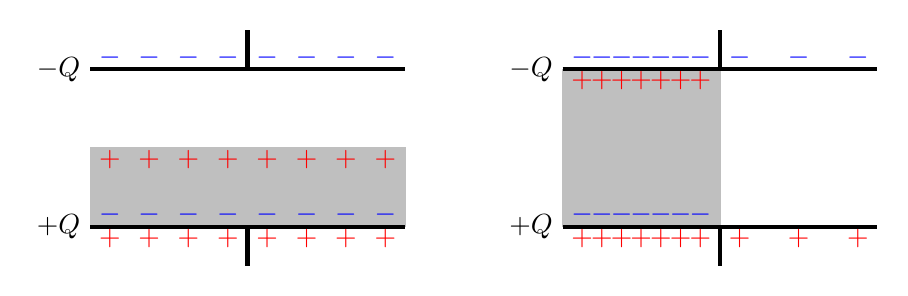
\begin{tikzpicture}
            \tikzstyle{wire} = [ultra thick]
            \tikzstyle{dielectric} = [fill=lightgray, color=lightgray]
            \tikzstyle{positive} = [color=red]
            \tikzstyle{negative} = [color=blue]
            \draw[dielectric] (0, 0) rectangle (4, 1);
            \draw[wire] (0, 0) -- (4, 0);
            \draw[wire] (0, 2) -- (4, 2);
            \draw[wire] (2, 0) -- (2, -0.5);
            \draw[wire] (2, 2) -- (2, 2.5);
            \node[left] at (0, 0) {\(+Q\)};
            \node[left] at (0, 2) {\(-Q\)};
            \foreach \x in {0.25, 0.75, ..., 3.75} {
                \node[positive] at (\x, 0.85) {\(+\)};
                \node[positive] at (\x, -0.15) {\(+\)};
                \node[negative] at (\x, 0.15) {\(-\)};
                \node[negative] at (\x, 2.15) {\(-\)};
            }
            
            \begin{scope}[xshift=6cm]
                \draw[dielectric] (0, 0) rectangle (2, 2);
                \draw[wire] (0, 0) -- (4, 0);
                \draw[wire] (0, 2) -- (4, 2);
                \draw[wire] (2, 0) -- (2, -0.5);
                \draw[wire] (2, 2) -- (2, 2.5);
                \node[left] at (0, 0) {\(+Q\)};
                \node[left] at (0, 2) {\(-Q\)};
                \foreach \x in {0.25, 0.5, ..., 1.75} {
                    \node[positive] at (\x, 1.85) {\(+\)};
                    \node[positive] at (\x, -0.15) {\(+\)};
                    \node[negative] at (\x, 0.15) {\(-\)};
                    \node[negative] at (\x, 2.15) {\(-\)};
                }
                \foreach \x in {2.25, 3, 3.75} {
                    \node[positive] at (\x, -0.15) {\(+\)};
                    \node[negative] at (\x, 2.15) {\(-\)};
                }
            \end{scope}
        \end{tikzpicture}
        \caption{The two interesting ways to half fill a capacitor with dielectric.}
        \label{fig:half filled capacitor}
    \end{figure}
    For the case of the capacitor half filled as shown on the left the addition of the dielectric does not break the planar symmetry of the situation and therefore \(\sigma_f\) is homogeneous.
    The high symmetry allows us to apply Gauss' law in media and from this we can get the displacement field and then from that we can get quantities of interest such as the electric field, polarisation field, bound charge density, potential, etc.
    For the case of the capacitor half filled as shown on the right the planar symmetry is broken and this means that Gauss' law is not as useful.
    By the symmetry of the situation we know that within the two regions, in the dielectric and outside the dielectric, the electric field is homogeneous.
    The free charge density, \(\sigma_f\), is inhomogeneous as the polarisation field distorts it.
    We therefore need to take a different approach to find the electric field we can construct equipotentials and then from the electric field we can find the displacement field and other interesting quantities.
    
    \section{The Magnetic Field in Media}
    \subsection{Types of Magnetisation}
    When an external magnetic field is applied to a material it will produce a magnetisation response.
    There are three mechanisms by which this can happen:
    \begin{itemize}
        \item Diamagnetism -- All materials have a diamagnetic response but it is only important in materials without an intrinsic magnetic moment as it is such a weak effect.
        What happens is the external magnetic field alters the angular momentum of the electrons which induces a field that opposes the external field.
        
        \item Paramagnetism -- This effect is important in materials in which each atom/molecule has an intrinsic magnetic moment and they are free to move.
        When an external field is applied these individual magnetic moments align with the field and create an induced field parallel to the applied field.
        
        \item Ferromagnetism -- This effect occurs in only a few materials.
        In these materials the intrinsic magnetic moments of individual species can align and stay aligned.
        However this is a local effect and the material will become a mosaic of `domains' where in each domain the magnetic moments of all species are aligned.
        When an external field is applied the domain boundaries will change in a way that favours domains where the magnetic moment is aligned with the external field.
        When the magnetic field is removed the domain boundaries do not return to where they where.
        This is the process by which a permanent magnet can be created.
    \end{itemize}
    
    \subsection{Magnetisation Field}
    The \define{magnetisation field}, \(\vv{M}\), is the net magnetisation dipole density in volume \(\dd{V}\):
    \[\dd{\vv{m}} = \vv{M}\dd{V}\]
    where \(\dd{\vv{m}}\) is the neg magnetic dipole moment due to the material in \(\dd{V}\).
    This is analogous to the definition of \(\vv{P}\) in section~\ref{sec:dielectric materials}.
    
    We can think of the magnetic dipole at a point as being the result of a small current loop.
    These then combine to give a macroscopic effect.
    \begin{figure}
        \centering
        \tikzsetnextfilename{net-magnetic-moment}
        \begin{tikzpicture}
            \draw[fill=lightgray, color=lightgray] (0, 0)  rectangle (4, 4);
            \foreach \x in {0, 1, 2, 3} {
                \foreach \y in {0, 1, 2, 3} {
                    \draw[ultra thick] ($(\x, \y) + (0.5, 0.5)$) circle[radius=0.35cm];
                    \draw[ultra thick, ->] ($(\x, \y) + (0.85, 0.501)$) -- ($(\x, \y) + (0.85, 0.499)$);
                }
            }
            \foreach \x in {-0.5, 0.5, ..., 4.5} {
                \foreach \y in {-0.5, 0.5, ..., 4.5} {
                    \node[color=red] at (\x, \y) {\(\otimes\)};
                }
            }
            \node[color=red, above right] at (4.5, 4.5) {\(\vv{B}\)};
            
            \begin{scope}[xshift=1cm]
                \draw[fill=lightgray, ultra thick] (6, 0) rectangle (10, 4);
                \draw[ultra thick, ->] (10, 2.01) -- (10, 1.99);
                \draw[ultra thick, ->] (6, 1.99) -- (6, 2.01);
                \foreach \x in {5.5, 6.5, ..., 10.5} {
                    \foreach \y in {-0.5, 0.5, ..., 4.5} {
                        \node[color=red] at (\x, \y) {\(\otimes\)};
                    }
                }
                \node[color=red, above right] at (10.5, 4.5) {\(\vv{B}\)};
            \end{scope}
        \end{tikzpicture}
        \caption{Individual magnetic moments viewed as microscopic current loops vs. the net magnetic moment viewed as a macroscopic current loop.}
        \label{fig:magnetisation due to homogenous magnetic field}
    \end{figure}
    Figure~\ref{fig:magnetisation due to homogenous magnetic field} shows the net effect of many individual magnetic moments.
    In this case the magnetic field is homogenous and this results in there being no current in the material, \(\vv{J_M} = \vv{0}\).
    There is only a surface current, \(\vv{j_M}\).
    If the field were not homogenous then there would be an internal current.
    The magnetic moments for an inhomogeneous magnetic field are shown in figure~\ref{fig:magnetisation due to inhomogeneous magnetic field}
    \begin{figure}[ht]
        \centering
        \tikzsetnextfilename{inhomogeneous-net-magnetic-moment}
        \begin{tikzpicture}
            \draw[color=lightgray, fill=lightgray] (0, 0) rectangle (4, 4);
            \foreach \y in {-0.5, 0.5, ..., 4.5} {
                \node[color=red] at (-0.5, \y) {\scriptsize \(\otimes\)};
                \node[color=red] at (0.5, \y) {\footnotesize \(\otimes\)};
                \node[color=red] at (1.5, \y) {\small \(\otimes\)};
                \node[color=red] at (2.5, \y) {\normalsize \(\otimes\)};
                \node[color=red] at (3.5, \y) {\large \(\otimes\)};
                \node[color=red] at (4.5, \y) {\Large \(\otimes\)};
            }
            \node[above right, color=red] at (4.5, 4.5) {\(\vv{B}\)};
            \foreach \y in {0.5, 1.5, ..., 3.5} {
                \draw[ultra thick] (0.5, \y) circle[radius=0.2cm];
                \draw[ultra thick, ->] ($(0.7, \y) + (0, 0.001)$) -- ($(0.7, \y) - (0, 0.001)$);
                \draw[ultra thick] (1.5, \y) circle[radius=0.25cm];
                \draw[ultra thick, ->] ($(1.75, \y) + (0, 0.001)$) -- ($(1.75, \y) - (0, 0.001)$);
                \draw[ultra thick] (2.5, \y) circle[radius=0.3cm];
                \draw[ultra thick, ->] ($(2.8, \y) + (0, 0.001)$) -- ($(2.8, \y) - (0, 0.001)$);
                \draw[ultra thick] (3.5, \y) circle[radius=0.35cm];
                \draw[ultra thick, ->] ($(3.85, \y) + (0, 0.001)$) -- ($(3.85, \y) - (0, 0.001)$);
            }
        \end{tikzpicture}
        \caption{Individual magnetic moments due to an inhomogeneous magnetic field.}
        \label{fig:magnetisation due to inhomogeneous magnetic field}
    \end{figure}
    In this case the eddy currents do not cancel and we have an internal current, \(\vv{J_M}\), as well as the surface current, \(\vv{j_M}\).
    
    We now want to quantify these effects.
    To do this we use the magnetic vector potential at \(\vv{r}\) due to an ideal magnetic dipole, \(\vv{m}\), at \(\vv{r'}\):
    \[\vv{A}(\vv{r}) = \frac{\mu_0}{4\pi} \frac{\vv{m}\times (\vv{r} - \vv{r'})}{\abs{\vv{r} - \vv{r'}}^3}.\]
    This generalises by superposition to
    \[\vv{A}(\vv{r}) = \frac{\mu_0}{4\pi} \int_V \frac{\vv{M}\times (\vv{r} - \vv{r'})}{\abs{\vv{r} - \vv{r'}}^3}\dd[3]{r'}.\]
    We then use the identity
    \[\frac{\vv{r} - \vv{r'}}{\abs{\vv{r} - \vv{r'}}^3} = \grad' \frac{1}{\abs{\vv{r} - \vv{r'}}}\]
    where \(\grad'\) is the gradient operator that acts only on \(\vv{r'}\).
    Hence
    \[\vv{A}(\vv{r}) = \frac{\mu_0}{4\pi} \int_V \vv{M}(\vv{r'}) \times \grad'\left[\frac{1}{\abs{\vv{r} - \vv{r'}}}\right] \dd[3]{r'}.\]
    We then use the product rule, \(\curl(f\vv{K}) = f\curl\vv{K} - \vv{K}\times\grad f\), to get
    \begin{align*}
        \vv{A}(\vv{r}) &= \frac{\mu_0}{4\pi} \int_V \frac{\grad'\times\vv{M}(\vv{r'})}{\abs{\vv{r} - \vv{r'}}} \dd[3]{r'} - \frac{\mu_0}{4\pi} \int_V \curl\left[\frac{\vv{M}(\vv{r'})}{\abs{\vv{r} - \vv{r'}}}\right] \dd[3]{r'}\\
        &= \frac{\mu_0}{4\pi} \int_V \frac{\grad'\times\vv{M}(\vv{r'})}{\abs{\vv{r} - \vv{r'}}} \dd[3]{r'} - \frac{\mu_0}{5\pi} \oint_S \left[\frac{\vv{M(\vv{r'})}}{\abs{\vv{r} - \vv{r'}}}\right]\times \dd{\vv{S'}}.
    \end{align*}
    Recall that
    \[\laplacian\vv{A} = \mu_0\vv{J} \implies \vv{A} = \frac{\mu_0}{4\pi} \int_V \frac{\vv{J}(\vv{r'})}{\abs{\vv{r} - \vv{r'}}}\dd[3]{r'}.\]
    This allows us to interpret the numerators of both integrands as currents.
    First
    \[\vv{J_M} = \curl\vv{M}\]
    is the bulk magnetisation current density, second
    \[\vv{j_M} = \vv{M}\times\vh{n}\]
    is the surface current density where \(\vh{n}\) is normal to the surface \(S'\) which bounds the volume \(V'\).
    
    \begin{example}
        A cylindrical bar magnet has uniform magnetisation, \(M\), along its axis.
        To what current distribution is this equivalent?
        
        \(\vv{M}\) is uniform so \(\curl\vv{M} = \vv{0}\) meaning \(\vv{J_M} = 0\).
        The surface current density is then
        \[\vv{j_M} = \vv{M}\times\vh{n} = M\ve{z}\times\ve{\rho} = M\ve{\varphi}.\]
        This has magnitude \(M\) and is `solenoidal', i.e. it resembles a solenoid with current flow around the circumference of a cylinder.
    \end{example}
    \begin{example}
        A long cylindrical bar magnet of uniform magnetisation is bent into a loop.
        To what current distribution is this equivalent?
        
        The curl in cylindrical coordinates is
        \[\curl\vv{M} = \left[\frac{1}{\rho}\pdv{M_z}{\varphi} - \pdv{M_\varphi}{z}\right]\ve{\rho} + \left[\pdv{M_\rho}{z} - \pdv{M_z}{\rho}\right]\ve{\varphi} + \frac{1}{\rho}\left[\pdv{\rho}(\rho M_\varphi) - \pdv{M_\rho}{\varphi}\right]\ve{z}.\]
        With this setup \(\vv{M}\) is circumferential so \(\vv{M} = M\ve{\varphi}\) so \(M_\rho = M_z = 0\) meaning that the curl reduces to
        \[\curl\vv{M} = \frac{1}{\rho}\pdv{\rho}(\rho M) = \frac{M}{\rho}\ve{z} = \vv{J_M}.\]
        The surface current has magnitude \(M\) and wraps around the cylinder still.
        The surface current is `toroidal', i.e. it resembles a toroidal solenoid with current flow over the surface.
        The bulk current density makes up for the fact that due to the geometry the net surface current is greater on the outside of the torus than the inside due to the greater surface area.
    \end{example}
    
    \subsection{Amp\`ere's Law in Media}
    The Amp\`ere--Maxwell law in a vacuum is
    \[\curl\vv{B} = \mu_0(\vv{J} + \varepsilon\partial_t\vv{E}).\]
    We divide \(\vv{J}\) into three parts: \(\vv{J_f}\) which is the current due to free charges, this is the normal current with which we have dealt so far, \(\vv{J_M} = \curl\vv{M}\) which is the magnetisation current as defined in the previous section, and \(\vv{J_P}\) which is the polarisation current which accounts for the movement of electric dipoles.
    To rationalise the introduction of \(\vv{J_P}\) we define a new charge density, \(\rho_P = -\div\vv{P}\), which follows the continuity equation
    \[\partial_t \rho_P + \div\vv{J_P} = 0.\]
    From this we have
    \[\vv{J_P} = \partial_t\vv{P}.\]
    We aim to write the Amp\`ere--Maxwell law in terms of \(\vv{J_f}\) only:
    \begin{align*}
        \curl\vv{B} &= \mu_0 (\vv{J_f} + \vv{J_M} + \vv{J_P} + \varepsilon_0\partial_t\vv{E})\\
        &= \mu_0(\vv{J_f} + \curl\vv{M} + \partial_t\vv{P} + \varepsilon_0\partial_t\vv{E})\\
        &= \mu_0(\vv{J_f} + \curl\vv{M} + \partial_t\vv{D})
    \end{align*}
    From this we have
    \[\curl\left[\frac{1}{\mu_0}\vv{B} - \vv{M}\right] = \vv{J_f} + \partial_t\vv{D}.\]
    We then define
    \[\vv{H} = \frac{1}{\mu_0}\vv{B} - \vv{M}\]
    so
    \[\curl\vv{H} = \vv{J_f} + \partial_t\vv{D}.\]
    This is the Amp\`ere--Maxwell law in media.
    In integral form it reads
    \[\oint_C \vv{H}\cdot\dd{\vv{l}} = \int_S (\vv{J_f} + \partial_t\vv{D})\cdot\dd{\vv{S}} = I_{f, \enc},\]
    where \(C\) is the contour bounding the surface \(S\).
    
    Confusingly \(\vv{H}\) is often referred to as the `magnetic field' and so is \(\vv{B}\).
    In some texts \(\vv{B}\) is the `magnetic flux density' and \(\vv{H}\) is the `magnetic field strength' but in other texts \(\vv{B}\) is the `magnetic field' and \(\vv{H}\) is the `auxiliary field'.
    For this reason it is best to specify `the magnetic \(\vv{B}\) field' or `the magnetic \(\vv{H}\) field'.
    
    Maxwell's second and third laws do not need modification in media as they contain no source terms, \(\rho\) or \(\vv{J}\).
    This means that we now have the four Maxwell equations in media:
    \begin{align*}
        \div\vv{D} &= \rho_f \tag{MI in media}\\
        \div\vv{B} &= 0 \tag{MII}\\
        \curl\vv{E} &= -\partial_t\vv{B} \tag{MIII}\\
        \curl\vv{H} &= \vv{J_f} + \partial_t\vv{D} \tag{MIV in media}
    \end{align*}
    
    We define the \define{magnetic susceptibility}, \(\chi_M\), to describe the relationship between \(\vv{M}\) and \(\vv{H}\):\footnote{some texts use \(\chi_B\vv{B} = \mu_0\vv{M}\) instead, these are related by \(\chi_B = \chi_M/(1 + \chi_M)\)}
    \[\vv{M} = \chi_M\vv{H}.\]
    In general \(\chi_M\) is a tensor however in \gls{lih} media it is a scalar.
    From this we also have
    \[\vv{B} = \mu_r\mu_0\vv{H} = \mu_0(1 + \chi_M)\vv{H} = \mu\vv{H}\]
    where \(\mu_r = 1 + \chi_M\) is the \define{relative permeability} and \(\mu = \mu_0\mu_r\) is the \define{absolute permeability}.
    In the absence of magnetisation \(\chi_M = 0\) and \(\mu_r = 1\).
    Unlike with dielectrics \(\chi_M\) can be positive or negative and consequently \(\mu_r\) is unbounded.
    For example a diamagnetic material will have \(\chi_M < 0\) whereas a paramagnetic material will have \(\chi_M > 0\) which corresponds to the fact that the fields induced in these two materials will be in opposite directions.
    
    \subsection{Media in Solenoids}
    A solenoid is filled with \gls{lih} medium with magnetic susceptibility \(\chi_M\).
    What is the effect compared to a solenoid containing a vacuum?
    
    The magnetisation field is given by \(\vv{M} = \chi_M\vv{H}\).
    The inductance of a solenoid is given by \(L = \Phi_B/I\).
    We first get \(\vv{H}\) from
    \[\curl\vv{H} = \vv{J_f} + \partial_t\vv{D} \implies \oint_C \vv{H}\cdot\dd{\vv{l}} = I_{f, \enc}.\]
    By symmetry we know that \(\vv{H}\) is axial and constant inside the solenoid and zero outside the solenoid.
    Thus if we define an Amp\'erian loop we only need integrate along the part inside the solenoid parallel to the axis.
    If this part has length \(l\) then
    \[\oint_C\vv{H}\cdot\dd{\vv{l}} = Hl = I_{f, \enc} = nlI \implies H_z = nI\]
    where \(n\) is the number of loops the solenoid has per unit length.
    From this we have
    \[\vv{B} = \mu_0\mu_r\vv{H} = \mu_0(1 + \chi_M)hI\ve{z}.\]
    This allows us to calculate the flux through the inductor treating the inductor as \(n\) loops of area \(A\) per unit length we have
    \[\Phi_B = ABnl = \mu_0(1 + \chi_M)n^2AlI\]
    where \(A\) is the cross sectional area of the solenoid.
    So the inductance is
    \[L = \frac{\Phi_B}{I} = \mu_0(1 + \chi_M)n^2Al = \mu_0(1 + \chi_M)n^2V_s\]
    where \(V_s = Al\) is the volume of the solenoid.
    
    \subsubsection{Partially Filled Solenoids}
    There are two interesting ways to half fill a solenoid.
    The first is with a cylindrical core which has a radius smaller than the solenoid.
    This preserves the cylindrical symmetry and therefore we can use Amp\`ere's law with two different cases, one that reaches all the way to the media and the other which stops in the vacuum.
    
    The second is with a cylindrical core that is of the same radius as the solenoid but doesn't extend for the solenoids entire length.
    This breaks the cylindrical symmetry.
    We can view this as two contributions, one from the filled section and one from the empty section.
    We cannot use Amp\`ere's law in this scenario to find the field.
    
    \section{Electromagnetism in Media}
    \subsection{Summary}
    Maxwell's equations for the macroscopic fields, \(\vv{D}\), \(\vv{B}\), \(\vv{E}\), and \(\vv{H}\), in media with free charge density, \(\rho_f\), and free current density, \(\vv{J_f}\), are
    \begin{align*}
        \div\vv{D} &= \rho_f, \tag{MI in media}\\ 
        \div\vv{B} &= 0, \tag{MII}\\
        \curl\vv{E} &= -\partial_t\vv{B},\tag{MIII}\\
        \curl\vv{H} &= \vv{J_f} + \partial_t\vv{D},\tag{MIV in media}
    \end{align*}
    Where the fields, \(\vv{D}\) and \(\vv{H}\), are defined as
    \[\vv{D} = \varepsilon_0\vv{E} + \vv{P},\qquad\text{and}\qquad \vv{B} = \mu_0(\vv{H} + \vv{M}).\]
    The free charges and currents satisfy the continuity equation
    \[\partial_t\rho_f + \div\vv{J_f} = 0.\]
    In \gls{lih} media the relations between the fields are
    \[\vv{P} = \chi_E\varepsilon_0\vv{E}, \qquad \vv{M} = \chi_M\vv{H}, \qquad \vv{D} = \varepsilon_0\varepsilon_r\vv{E} = \varepsilon\vv{E},\]
    \[\text{and}\qquad \vv{B} = \mu_0\mu_r\vv{H} = \mu\vv{H}.\]
    Where \(\varepsilon_r = 1 + \chi_E\) and \(\mu_r = 1 + \chi_M\).
    
    \subsection{Energy Density and the Poynting Vector}
    The power delivered by an \gls{em} field to a system of charge carriers is \(\vv{E}\cdot\vv{J_f}\) per unit volume.
    This means that the energy density, \(u\), obeys
    \[\dv{u}{t} = \vv{E}\cdot\vv{J_f}.\]
    We aim to express \(\vv{J_f}\) in field related quantities.
    First we use Maxwell's fourth law to write
    \[\vv{E}\cdot\vv{J_f} = \vv{E}\cdot\left[\curl\vv{H} - \partial_t\vv{D}\right] = \vv{E}\cdot(\curl\vv{H}) - \vv{E}\cdot\partial_t\vv{D}.\]
    We then use the product rule,
    \[\div(\vv{E}\times\vv{H}) = \vv{H}\cdot(\curl\vv{E}) - \vv{E}\cdot(\curl\vv{H}) \implies \vv{E}\cdot(\curl\vv{H}) - \vv{E}\cdot(\curl\vv{H}) - \div(\vv{E}\times\vv{H}),\]
    to get
    \[\vv{E}\cdot\vv{J} = \vv{H}\cdot(\curl\vv{E}) - \div(\vv{E}\times\vv{H}) - \vv{E}\cdot\partial_t\vv{D}.\]
    Using Maxwell's third law this becomes
    \[\vv{E}\cdot\vv{J_f} = -\vv{H}\cdot\partial_t\vv{B} - \div(\vv{E}\times\vv{H}) - \vv{E}\cdot\partial_t\vv{D}.\]
    Next we use that in \gls{lih} media
    \[\vv{E}\cdot\partial_t\vv{D} = \vv{E}\cdot\partial_t(\varepsilon\vv{E}) = \varepsilon\vv{E}\cdot\partial_t\vv{E} = \vv{D}\cdot\partial_t\vv{E}\]
    and
    \[\vv{H}\cdot\partial_t\vv{B} = \mu\vv{B}\cdot\partial_t\vv{B} = \vv{B}\cdot\partial_t(\mu\vv{B}) = \vv{B}\cdot\partial_t\vv{H}.\]
    This gives us
    \[\vv{E}\cdot\vv{J_f} = -\vv{B}\cdot\partial_t\vv{H} - \vv{D}\cdot\partial_t\vv{E} - \div(\vv{E}\times\vv{H}).\]
    Recognising the standard product rule
    \[\partial_t(\vv{E} \cdot \vv{D}) = \vv{D}\cdot\partial_t\vv{E} + \vv{E}\cdot\partial_t\vv{D} = 2\vv{D}\cdot\partial_t\vv{E}\]
    and similarly for the magnetic fields this becomes
    \[\vv{E}\cdot\vv{J_f} = \frac{1}{2}\partial_t(\vv{E}\cdot\vv{D} + \vv{B}\cdot\vv{H}).\]
    We then integrate over a volume, \(V\), to get the energy from the energy density.
    Using the divergence theorem on the second term we get
    \[\dv{U}{t} = -\frac{1}{2}\dv{t}\int_V (\vv{E}\cdot\vv{D} + \vv{B}\cdot\vv{H})\dd{V} - \oint_A(\vv{E}\times\vv{H})\cdot\dd{\vv{A}}.\]
    We now identify the electric and magnetic energy densities as
    \[u_E = \frac{1}{2}\vv{E}\cdot\vv{D}, \qquad\text{and}\qquad u_M = \frac{1}{2}\vv{B}\cdot\vv{H}\]
    respectively.
    From the second term we identify the macroscopic Poynting vector as
    \[\vv{S} = \vv{E}\times\vv{H}\]
    so the power delivered to the charges can be written as
    \[\dv{U}{t} = -\dv{t}[U_E + U_M] - \oint_A\vv{S}\cdot\dd{\vv{A}}.\]
    
    \subsection{Boundary Conditions}
    \subsubsection{Qualitatively}
    Now that we have characterised fields in and out of media we want to know how the fields behave at the boundary between media.
    To do this we use the work we have done already with half filled capacitors/inductors and we make the unjustified assumption that the same analysis holds outside of a capacitor/inductor.
    Figure~\ref{fig:fields at boundaries} shows qualitatively what happens at a boundary for the four fields, this figure assumes that \(\chi_M > 0\).
    The two cases we consider for each field are what happens to the tangential component and the normal component at the boundary.
    \begin{figure}[ht]
        \centering
        \tikzsetnextfilename{fileds-boundary-conditions}
        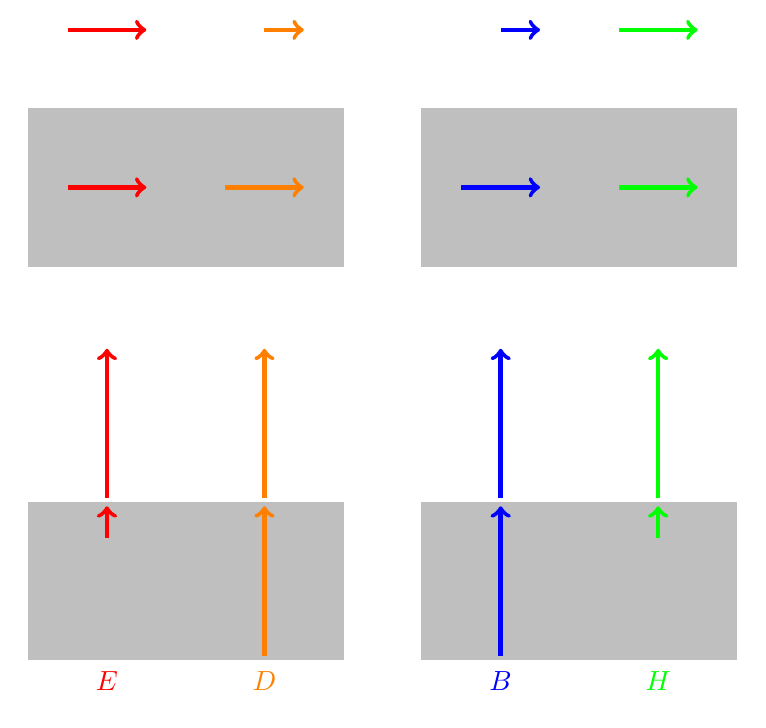
\begin{tikzpicture}
            \tikzstyle{media} = [fill=lightgray, color=lightgray]
            \tikzstyle{field} = [ultra thick, ->]
            \tikzstyle{E} = [field, color=red]
            \tikzstyle{B} = [field, color=blue]
            \tikzstyle{D} = [field, color=orange]
            \tikzstyle{H} = [field, color=green]
            \draw[media] (0, 0) rectangle (4, 2);
            \draw[media] (5, 0) rectangle (9, 2);
            \draw[media] (0, 5) rectangle (4, 7);
            \draw[media] (5, 5) rectangle (9, 7);
            \draw[E] (1, 1.55) -- (1, 1.95);
            \draw[E] (1, 2.05) -- (1, 3.95);
            \draw[D] (3, 0.05) -- (3, 1.95);
            \draw[D] (3, 2.05) -- (3, 3.95);
            \draw[E] (0.5, 6) -- (1.5, 6);
            \draw[E] (0.5, 8) -- (1.5, 8);
            \draw[D] (2.5, 6) -- (3.5, 6);
            \draw[D] (3, 8) -- (3.5, 8);
            \draw[B] (6, 0.05) -- (6, 1.95);
            \draw[B] (6, 2.05) -- (6, 3.95);
            \draw[H] (8, 1.55) -- (8, 1.95);
            \draw[H] (8, 2.05) -- (8, 3.95);
            \draw[B] (5.5, 6) -- (6.5, 6);
            \draw[B] (6, 8) -- (6.5, 8);
            \draw[H] (7.5, 6) -- (8.5, 6);
            \draw[H] (7.5, 8) -- (8.5, 8);
            
            \node[below, E] at (1, 0) {\(\vv{E}\)};
            \node[below, D] at (3, 0) {\(\vv{D}\)};
            \node[below, B] at (6, 0) {\(\vv{B}\)};
            \node[below, H] at (8, 0) {\(\vv{H}\)};
        \end{tikzpicture}
        \caption{The qualitative behaviour of fields at a boundary between media. The normal and tangential components of the four fields are shown both in the media and outside.}
        \label{fig:fields at boundaries}
    \end{figure}
    \subsubsection{Quantitatively}
    We can be much more rigorous if we use Maxwell's laws.
    We assume we have a plane and above and below the plane are two different media, media 1 below and media 2 above.
    We use a Gaussian surface that is a cylindrical pill box of height \(h\) with the flat faces parallel to the plane, and a rectangular Amp\'erian loop of height \(h\) with two sides running parallel to the plane.
    We also define two vectors, \(\vh{n}\), and \(\vh{t}\), which are normal and tangential to the plane respectively.
    
    The first condition we consider is Maxwell's first law,
    \[\div\vv{D} = \rho_f.\]
    From this and the divergence theorem we have
    \[\oint_S\vv{D}\cdot\dd{\vv{S}} = Q_{f, \enc}.\]
    pill box has a surface normal, on the flat faces, of \(\dd{\vv{S}} = \vh{n}\dd{S}\).
    Allowing \(h\to 0\) we can ignore the contribution to the integral from the sides of the pill box and we get
    \[\int\vv{D}\cdot\dd{\vv{S}} = \int(\vv{D_2} - \vv{D_1})\cdot\vh{n}\dd{S} = \int \sigma_f \dd{S}\]
    where the last equality arises from the definition of a surface charge density.
    Note that \(\vv{D_1}\) is the \(\vv{D}\) field below the plane and \(\vv{D_2}\) is the \(\vv{D}\) field above the plane.
    Since both integrals are over the same area we can conclude that
    \[(\vv{D_2} - \vv{D_1})\cdot\vh{n} = \sigma_f.\]
    Taking the scalar product with \(\vh{n}\) picks out the scalar component of \(\vv{D_2} - \vv{D_1}\) and so \(\vv{D_{\mathrm{normal}}}\) is continuous \emph{if and only if} \(\sigma_f = 0\).
    
    The second condition we consider is Maxwell's second law,
    \[\div\vv{B} = 0 \implies \oint_S \vv{B}\cdot\dd{\vv{S}} = 0.\]
    Using the same Gaussian surface and again allowing \(h\to 0\) we have
    \[\int\vv{B}\cdot\dd{\vv{S}} = \int (\vv{B_2} - \vv{B_1})\cdot\vh{n}\dd{S} = 0.\]
    This holds for any similarly defined surface so
    \[(\vv{B_2} - \vv{B_1})\cdot\vh{n} = 0\]
    meaning that \(\vv{B_{\mathrm{normal}}}\) is \emph{always} continuous.
    
    The third condition we consider is Maxwell's third law,
    \[\curl\vv{E} = -\partial_t\vv{B} \implies \oint_C\vv{E}\cdot\dd{\vv{l}} = -\partial_t\Phi_B.\]
    We use an Amp\'erian loop of length \(\ell\) and height \(h\).
    Allowing \(h\to -\) we also have \(\Phi_B\to 0\) as long as \(B\) is finite.
    Therefore
    \[\int \vv{E}\cdot\dd{\vv{l}} = \int(\vv{E_2} - \vv{E_1})\cdot\vh{t} \dd{l} = 0\]
    where \(\vh{t}\) is tangential to the surface meaning that \(\vh{t}\cdot\vh{n} = 0\).
    Since this holds no matter where we put the Amp\'erian loop, or define \(\vh{t}\) we have
    \[(\vv{E_2} - \vv{E_1})\cdot\vh{t} = 0\]
    meaning that \(\vv{E_{\mathrm{tangential}}}\) is \emph{always} continuous.
    
    The final condition that we consider is Maxwell's fourth law
    \[\curl\vv{H} = \vv{J_f} + \partial_t\vv{D}\]
    in integral form this becomes
    \[\oint_{C}\vv{H}\cdot\dd{\vv{l}} = \vv{j_f} \cdot \vh{s}\ell + (\partial_t\vv{D})\cdot\vh{s}\ell h\]
    where \(\vv{j_f}\) is the free surface current per unit area and \(\vh{s} = \vh{t}\times\vh{n}\) is the surface unit vector perpendicular to the Amp\'erian loop.
    Now allowing \(h\to 0\) we have
    \[\int\vv{H}\cdot\dd{\vv{l}} = \vv{H_1} - \vv{H_2})\cdot\vh{t}\ell = \vh{j_f}\cdot\vh{s}\ell.\]
    Since \(\vh{n}\) is normal to the plane \(\vh{s}\) is tangential to the plane so \(\vv{H_\mathrm{tangential}}\) is continuous \emph{if and only if} \(\vv{j_f} = \vv{0}\).
    This general form can be written in other ways, including
    \begin{align*}
        (\vv{H_1} - \vv{H_2})\cdot\vh{t} &= \vv{j_f}\cdot\vh{s},\\
        (\vv{H_{2, \mathrm{tangential}}} - \vv{H_{1, \mathrm{tangential}}}) &= \vv{j_f}\times\vh{n},\\
        (\vv{H_2} - \vv{H_1})\times\vh{n} &= -\vv{j_f}.
    \end{align*}

    In summary at a boundary between media
    \begin{itemize}
        \item \(\vv{D_{\mathrm{normal}}}\) is continuous if and only if \(\sigma_f = 0\).
        \item \(\vv{B_{\mathrm{normal}}}\) is continuous always.
        \item \(\vv{E_{\mathrm{tangential}}}\) is continuous always.
        \item \(\vv{H_{\mathrm{tangential}}}\) is continuous if and only if \(\vv{j_f} = \vv{0}\).
    \end{itemize}

    \section{Continuity Conditions and Waves in Media}
    \subsection{Applications of Continuity Conditions}
    \subsubsection{Inclined Dielectric}
    Consider the setup in figure~\ref{fig:refraction}.
    \begin{figure}[ht]
        \centering
        \tikzsetnextfilename{refraction}
        \begin{tikzpicture}
            \tikzstyle{mid arrow} = [postaction={decorate, decoration={markings, mark=at position .5 with {\arrow{>}}}}]
            \tikzstyle{E base} = [ultra thick, color=red]
            \tikzstyle{E} = [E base, mid arrow]
            \tikzstyle{angle} = [very thick]
            \tikzstyle{media} = [color=lightgray, fill=lightgray]
            \tikzstyle{axis} = [very thick, ->]
            \draw[media] (-2, -2) rectangle (2, 0);
            \draw[axis] (0, -2) -- (0, 2) node[above] {\(z\)};
            \draw[E] (2, 2) -- (0, 0);
            \draw[E] (0, 0) -- (-1, -2);
            \draw[angle] (0.5, 0.5) arc[start angle=45, end angle=90, radius=0.707cm];
            \draw[angle] (0, -0.707) arc[start angle=-90, end angle=-116.6, radius=0.707cm];
            \node[below right, E base] at (1, 1) {\(\vv{E^o}\)};
            \node[left, E base] at (-0.5, -1) {\(\vv{E^i}\)};
            \node at (0.4, 0.8) {\(\vartheta\)};
            \node at (-0.2, -0.9) {\(\psi\)};
        \end{tikzpicture}
        \caption{An inclined dielectric with an incident electric field.}
        \label{fig:refraction}
    \end{figure}
    It shows a uniform electric field, \(\vv{E^o}\), incident on a dielectric at an angle \(\vartheta\).
    The field is then refracted and the field in the dielectric is at an angle \(\psi\).
    We want to know what the field, \(\vv{E^i}\), inside the dielectric is.
    
    Outside the dielectric we define the displacement field as
    \[\vv{D^o} = \varepsilon_0\vv{E^o}.\]
    Inside the dielectric the displacement field is
    \[\vv{D^i} = \varepsilon_0\varepsilon_r\vv{E^i}.\]
    We apply the boundary condition that the normal component of the displacement field, \(D_n\), is continuous at the boundary, since there is no surface charge.
    This means that \(D^o_z = D^i_z\).
    The second boundary condition is that the tangential components of the electric field, \(E_t\), are continuous at the boundary.
    This means that \(E^o_x = E^i_x\) and \(E^o_y = E^i_y\).
    We choose a coordinate system such that \(E^o_y = E^i_y = 0\) meaning that we can work in the two-dimensional \((x, z)\)-plane.
    In this plane the full fields are
    \[\vv{E^o} = (E^o\sin\vartheta, E^o\cos\vartheta), \qquad\text{and}\qquad \vv{E^i} = (E^i\sin\psi, E^i\cos\psi).\]
    Applying the first continuity condition we have
    \[D^o_z = D_i^z \implies \varepsilon_0E^o\cos\vartheta = \varepsilon_0\varepsilon_rE^i\cos\psi \implies E^i = \frac{1}{\varepsilon_r}E^o\frac{\cos\vartheta}{\cos\psi}.\]
    Applying the second continuity condition we have
    \[E^o_x = E^i_x \implies E^o\sin\vartheta = E^i\sin\psi \implies E^i = E^o\frac{\sin\vartheta}{\sin\psi}.\]
    Combining these we have
    \[\frac{1}{\varepsilon_r}\frac{\cos\vartheta}{\cos\psi} = \frac{\sin\vartheta}{\sin\psi} \implies \frac{\sin\psi}{\cos\psi} = \tan\psi = \varepsilon_r\frac{\sin\vartheta}{\cos\vartheta} = \varepsilon_r\tan\vartheta \implies \psi = \arctan(\varepsilon_r\tan\vartheta).\]
    It is worth checking two basic case here.
    First we consider the case when \(\vartheta = 0\).
    In this case \(\psi = \arctan(\varepsilon_r\tan 0) = \arctan 0 = 0\) and so there is no refraction which is what we would expect.
    Going a step further back in the calculation if \(\psi = \vartheta = 0\) then we recover that \(D^o_z = D^i_z\).
    The second case we consider is \(\vartheta = \pi/2\).
    In this case \(\psi = \arctan(\varepsilon_r\tan(\pi/2)) = \arctan(\infty) = \pi/2\) and so there is no refraction as the field travels along the boundary.
    Going a step further back in the calculation if \(\psi = \vartheta = \pi/2 \) then we recover \(E^o = E^i\).
    
    \subsubsection{Spherical Cavity in a Dielectric}
    Suppose we have a large block of \gls{lih} dielectric which contains a spherical cavity.
    The electric field far from the cavity is uniform and has magnitude \(E_0\).
    What are \(\vv{E}\) and \(\vv{D}\) in the cavity?
    
    We will use spherical coordinates with their origin at the centre of the cavity and aligned so that the \(z\)-axis is parallel to the field at large \(r\).
    See figure~\ref{fig:spherical cavity} for a diagram.
    \begin{figure}[ht]
        \centering
        \tikzsetnextfilename{spherical-cavity}
        \begin{tikzpicture}
            \tikzstyle{media} = [color=lightgray, fill=lightgray]
            \tikzstyle{E} = [->, ultra thick]
            \draw[media] (-3, -2) rectangle (3, 2);
            \draw[fill=white, color=white] (0, 0) circle[radius=1.5cm];
            \draw[dashed] (0, 0) -- (1.5, 0);
            \draw[dashed] (0, 0) -- (1.06, -1.06);
            \draw (0.5, 0) arc[start angle=0, end angle=-45, radius=0.5cm];
            \node at (-22.5:0.65) {\(\vartheta\)};
            \foreach \x in {0, -20, 20, 40, -40} {
                \node[color=red] at ($({-1*cos(\x)*1.65}, {sin(\x)*1.65})$) {\(+\)};
                \node[color=blue] at ($({cos(\x)*1.65}, {sin(\x)*1.65})$) {\(-\)};
            }
            \draw[E] (1.2, -1.6) -- (2.2, -1.6) node[right] {\(\vv{E_0}\)};
        \end{tikzpicture}
        \caption{A spherical cavity in a dielectric}
        \label{fig:spherical cavity}
    \end{figure}
    At the surface of the cavity a charge distribution, \(\sigma_P = \vv{P}\cdot\vh{n}\) forms.
    Note that \(\vh{n}\) is the outward normal of the dielectric, meaning it points \emph{towards} the origin.
    Since this is an \gls{lih} media \(\vv{P}\) is parallel to \(\vv{E}\) and so the field inside is enhanced by the charge distribution which is a function of the angle, \(\vartheta\), since \(r = 1.5\) on the surface of the cavity and the symmetry under changing \(\varphi\) means that \(\sigma_P\) cannot depend on \(\varphi\).
    
    The charge distribution, \(\sigma_P(\vartheta)\), forms an effective dipole.
    Outside of the cavity the field lines are locally distorted by this charge distribution.
    We want to determine \(V\), the electrostatic potential, and from this we can calculate \(\vv{E}\).
    Within the cavity we assume a uniform \(\vv{E}\) field in the \(z\) direction.
    This corresponds to a potential
    \[V(r) = -E_{\text{in}}z = -E_{\text{in}}r\cos\vartheta\]
    for \(r < a\) where \(a\) is the radius of the cavity.
    Outside of the cavity we use a superposition of a uniform \(\vv{E_0}\) field plus a dipole field so
    \[V(r) = -E_0r\cos\vartheta + \frac{A\cos\vartheta}{r^2}.\]
    Here \(A\) is a constant to be found which gives the relative strength of the dipole field.
    
    Thanks to the uniqueness theorem for Poisson's equation we need only show that this potential fulfils the boundary conditions and Poisson's equation and then we know that the electric field derived from this potential is unique.
    Since the charges are only on the boundary away from the boundary we only need the potential to satisfy Laplace's equation, \(\laplacian V = 0\).
    We then only need to check that the boundary conditions are satisfied.
    In spherical coordinates
    \[\grad V = \ve{r}\pdv{V}{r} + \ve{\vartheta}\frac{1}{r}\pdv{V}{\vartheta} + \ve{\varphi}\frac{1}{r\sin\vartheta}\pdv{V}{\vartheta} = -\vv{E}.\]
    The first boundary condition we check is that \(E_t\) is continuous.
    This requires \(E_\vartheta\) to be continuous at \(r = a\).
    So
    \[-E_0a\sin\vartheta + \frac{A\sin\vartheta}{a^2} = -E_{\text{in}}a\sin\vartheta.\]
    The second boundary condition is that \(D_n\) is continuous (note the surface density is due to polarisation, there is no free charge distribution).
    This requires \(D_r = \varepsilon_rE_r = -\varepsilon_r\partial_rV\) to be continuous.
    So
    \[\varepsilon_rE_o\cos\vartheta + \frac{2A\varepsilon_r\cos\vartheta}{a^3} = E_{\text{in}}\cos\vartheta.\]
    Combining these we have
    \[E_{\text{in}} = \varepsilon_r\left(E_0 + \frac{2A}{a^3}\right) = E_0 - \frac{A}{a^3}.\]
    Thus
    \[E_{\text{in}} = E_0\frac{3\varepsilon_r}{1 + 2\varepsilon_r}.\]
    Combining this with the requirement that \(\vv{E_{\mathrm{in}}} = E_{\mathrm{in}}\ve{z}\) and \(\vv{D_{\mathrm{in}}} = \varepsilon_0\vv{E_{\mathrm{in}}}\) (since inside the cavity \(\varepsilon_r = 1\)), we have the full field.
    Notice that \(E_{\text{in}} > E_0\) so the field in the cavity is stronger than the field outside.
    
    \subsection{Waves in Media}
    \subsubsection{Non-conduction Media}
    In a non-conducting media \(\rho_f = 0\) and \(\vv{J_f} = 0\).
    Thus
    \[\vv{D} = \varepsilon\vv{E}, \qquad\text{and}\qquad \vv{B} = \mu\vv{H}.\]
    We can derive macroscopic wave equations as before:
    \[\laplacian\vv{E} = \varepsilon\mu \pdv[2]{\vv{E}}{t}, \qquad\text{and}\qquad \laplacian\vv{B} = \varepsilon\mu\pdv[2]{\vv{B}}{t}.\]
    Clearly these have the normal plane wave solutions
    \[\vv{E} = \vv{E_0}e^{i(\vv{k}\cdot\vv{r} - \omega t)}, \qquad\text{and}\qquad \vv{B} = \vv{B_0}e^{i(\vv{k}\cdot\vv{r} - \omega t)}.\]
    Where \(k^2 = \mu\varepsilon\omega^2\).
    We interpret this as the wave phase velocity being
    \[v = \frac{\omega}{k} = \frac{1}{\sqrt{\mu\varepsilon}}.\]
    Recall that \(c = (\mu_0\varepsilon_0)^{-1/2}\) so
    \[v^2 = \frac{1}{\mu_r\varepsilon_r}c^2 = \frac{1}{n^2}c^2\]
    where we have defined \(n = \mu_r\varepsilon_r\) which is called the \define{refractive index} and is a property of the medium.
    As we did with waves in a vacuum it can be shown that
    \[i\vv{k}\cdot\vv{E_0} = 0, \qquad\text{and}\qquad i\vv{k}\cdot\vv{B_0} = 0.\]
    This means that \(\vv{E}\) and \(\vv{B}\) are perpendicular to the direction of propagation, \(\vv{k}\), and therefore the wave is transverse.
    We see that for \gls{lih} media all of the extra complications that come with having media are neatly hidden away in \(\varepsilon\) and \(\mu\) and have the net effect of changing the velocity of the wave.
    
    \subsubsection{Waves in Conductors}
    In conductors in general \(\rho_f \ne 0\) and \(\vv{J_f} \ne \vv{0}\).
    We will start with Ohm's law, \(\vv{J} = \sigma\vv{E}\) and assume linear media so
    \[\vv{D} = \varepsilon\vv{E}, \qquad\text{and}\qquad \vv{B} = \mu\vv{H}.\]
    Combining these with Maxwell's fourth equation gives us
    \begin{equation}\label{eqn:curl B}
        \curl\vv{H} = \vv{J_f} + \partial_t\vv{D} \implies \curl\vv{B} = \mu\sigma\vv{E} + \mu\varepsilon\partial_t\vv{E}.
    \end{equation}
    Taking the curl of Maxwell's third equation we have
    \[\curl(\curl\vv{E}) = \grad(\div\vv{E}) - \laplacian\vv{E} = -\curl(\partial_t\vv{B}) = -\partial_t(\curl\vv{B}).\]
    Substituting for \(\curl\vv{B}\) from equation~\ref{eqn:curl B} we have
    \[\partial_t\left(\mu\sigma\vv{E} + \mu\varepsilon\partial_t\vv{E}\right) = \laplacian\vv{E} - \grad\left(\frac{\rho}{\varepsilon}\right) = \laplacian\vv{E}\]
    where in the last equality we assume a uniform charge density meaning that \(\grad\rho = 0\).
    Rearranging this we have
    \[\laplacian\vv{E} = \mu\varepsilon\pdv[2]{\vv{E}}{t} + \mu\sigma\pdv{\vv{E}}{t}.\]
    Notice that this is the wave equation with an additional term on the right.
    The origin of this additional term is the free current.
    
    Taking the curl of Maxwell's fourth equation gives us
    \[\curl(\curl\vv{B}) = \grad(\div\vv{B}) - \laplacian\vv{B} = \mu\sigma\curl\vv{E} + \mu\varepsilon\partial_t(\curl\vv{E}).\]
    Substituting for Maxwell's second and third laws we have
    \[\laplacian\vv{B} =  \mu\varepsilon\partial_t\pdv[2]{\vv{B}}{t} + \mu\sigma\pdv{\vv{B}}{t}.\]
    
    \section{Waves In Conductors}
    We saw in the last section that we could derive wave equations in conductors which, if we assume linear media, have the form
    \[\laplacian\vv{E} = \mu\varepsilon\pdv[2]{\vv{E}}{t} + \mu\sigma\pdv{\vv{E}}{t}.\]
    We make the ansatz that this has the plane wave solution
    \[\vv{E} = \tilde{\vv{E}}e^{i(\tilde{k}z - \omega t)}\]
    where we assume the wave is travelling in the \(z\) direction.
    If we substitute this into the wave equation we get
    \[\tilde{k}^2 = \mu\varepsilon\omega^2 + i\mu\sigma\omega.\]
    This is the \define{dispersion relation}.
    To solve this we clearly need to consider some complex numbers.
    Let \(\tilde{k} = k + i\kappa\) for some \(k, \kappa\in\reals\).
    Then if we equate real and imaginary parts in the dispersion relation we have
    \[k^2 - \kappa^2 = \mu\varepsilon\omega^2, \qquad\text{and}\qquad 2k\kappa = \mu\sigma\omega.\]
    The second of these has the solution \(\kappa = \mu\sigma\omega/2k\) which allows us to eliminate \(\kappa\) from the first giving
    \[k^4 - \left(\frac{\mu\sigma\omega}{2}\right)^2 = \mu\varepsilon\omega^2k^2.\]
    This is a quadratic in \(k^2\) and has the solution
    \[k^2 = \frac{1}{2}\mu\varepsilon\omega^2 = \frac{1}{2}\left[(\mu\varepsilon\omega^2)^2 + (\mu\sigma\omega)^2\right]^{1/2} = \frac{\mu\varepsilon\omega^2}{2}\left[\left(1 + \left[\frac{\sigma}{\varepsilon\omega}\right]^2\right)^{1/2} + 1\right],\]
    where we choose the positive square root so that \(k^2\) is positive, since \(k\in\reals\).
    We can then use this to obtain
    \[\kappa^2 = \frac{\mu\varepsilon\omega^2}{2}\left[\left(1 + \left[\frac{\sigma}{\varepsilon\omega}\right]^2\right)^{1/2} - 1\right].\]
    Hence
    \[\vv{E} = \tilde{\vv{E_0}}e^{-\kappa z}e^{i(kz - \omega t)}.\]
    This describes exponential decay of the wave along \(z\), which is the propagation direction.
    The wave is attenuated over a characteristic distance, called the \define{skin depth}, which is given by
    \[\delta = \frac{1}{\kappa}.\]
    This gives the depth at which the amplitude of the wave is \(e^{-1}\) times the amplitude at which the wave enters the conductor.
    
    A good check to do here is consider the case when \(\sigma = 0\), this corresponds to a vacuum.
    In this case \(k^2 = \varepsilon\mu\omega^2\) and \(\kappa^2 = 0\) so we revert to the vacuum solution.
    
    \subsection{Good and Poor Conductors}
    The ratio \(\sigma/\varepsilon\omega\) is important in this result.
    Both \(1/\omega\) and \(\varepsilon/\sigma\) have units of time so this quantity is a ratio of two timescales.
    The question now is what do these timescales represent?
    
    Consider the continuity equation for free charges,
    \[\partial_t\rho_f + \div\vv{J_f} = 0.\]
    Using Ohm's law, \(\vv{J_f} = \sigma\vv{E}\) we have 
    \[\div\vv{J_f} = \sigma\div\vv{E} = \frac{\sigma}{\varepsilon}\div\vv{D} = \frac{\sigma}{\varepsilon}\rho_f\]
    so the continuity equation becomes
    \[\partial_t\rho_f = -\frac{\sigma}{\varepsilon}\rho_f.\]
    This has as a solution
    \[\rho_f(t) = \rho_f(0)e^{-\sigma t/\varepsilon}.\]
    So \(\varepsilon/\sigma\) is the characteristic timescale for how fast charge decays in a conductor.
    This is known as the \define{relaxation time}, \(\tau\).
    This quantity tells us how fast charges migrate to the surface and how fast the electric field disappears in a conductor.
    In an ideal conductor \(\sigma \to \infty\) and \(\tau \to 0\) which corresponds to our assumption for an ideal conductor that charge is always concentrated on the surface and \(\vv{E} = \vv{0}\) inside an ideal conductor.
    
    The interpretation of \(1/\omega\) is, as one would expect, the period of the wave, \(T = 2\pi/\omega\).
    Thus \(\sigma/\varepsilon\omega = T/2\pi\tau\).
    We use this ratio to characterise conductors as ``good" and ``bad".
    For a ``good" conductor \(\sigma/\varepsilon\omega \gg 1\).
    For a ``bad" conductor \(\sigma/\varepsilon\omega \ll 1\).
    Notice that how ``good" a conductor is depends on the frequencies that we care about transmitting.
    For example it is possible that a conductor can be a good conductor of radio waves, which have a relatively small value of \(\omega\), and a bad conductor of ultraviolet, which has a large value of \(\omega\).
   
    
    It can be shown that for a good conductor
    \[\delta \approx \sqrt{\frac{2}{\mu\omega\sigma}},\]
    and for a bad conductor
    \[\delta \approx \sqrt{\frac{4\varepsilon}{\mu\sigma^2}}.\]
    Typical metals are good conductors up to about \SI{1}{\mega\hertz} with \(\delta \approx \SI{1}{\centi\meter}\) at \SI{50}{\hertz} (mains power frequency) and \(\delta \approx \SI{10}{\micro\meter}\) at \SI{50}{\mega\hertz}.
    
    Some consequences of the skin depth are
    \begin{itemize}
        \item Cables greater than about \SI{1}{\centi\meter} in width are wasted as the current is mostly in the skin layer around the outside and there is a `dead zone' in the centre.
        Cables that initially seem thicker than \SI{1}{\centi\meter} are often actually multiple narrower cables bound together.
        \item Submarines cannot use radio as at the typical depth of a submarine radio waves simply cannot penetrate the water.
        \item Mobile phones don't work inside metal boxes as they use radio waves which have frequencies in the gigahertz range and therefore don't penetrate very far through metal.
        \item Microwave oven doors have a metal mesh with holes much smaller than the wavelength of the microwaves.
        This allows visible light through but not microwaves.
    \end{itemize}

    \subsection{Phase Relations of Fields}
    As with waves in a vacuum or insulator Maxwell's first and second laws imply that
    \[i\tilde{\vv{k}}\cdot\tilde{\vv{E_0}} = 0, \qquad\text{and}\qquad i\tilde{\vv{k}}\cdot\tilde{\vv{B_0}} = 0\]
    so the waves are transverse.
    In the case that \(\tilde{\vv{k}} = \tilde{k}\ve{z}\) and \(\tilde{\ve{E_0}} = \tilde{E_0}\ve{x}\) if we substitute into Maxwell's third equation we get
    \[i\tilde{\vv{k}}\times\tilde{\vv{E_0}} = i\omega\tilde{\vv{B_0}}\]
    hence
    \begin{equation}\label{eqn:B0 = kE0/omega ey}
        \tilde{\vv{B_0}} = \frac{\tilde{k}\tilde{E_0}}{\omega}\ve{y}.
    \end{equation}
    In general \(\tilde{k}\) is complex and therefore so are \(\tilde{E_0}\) and \(\tilde{B_0}\).
    We write
    \[\tilde{k} = Re^{i\varphi}, \qquad\text{where}\qquad R = \sqrt{k^2 + \kappa^2}, \qquad\text{and}\qquad \varphi = \arctan\left(\frac{\kappa}{k}\right).\]
    Then
    \[\tilde{E_0} = E_0e^{i\delta_E}, \qquad\text{and}\qquad \tilde{B_0} = B_0e^{i\delta_B}.\]
    Substituting these into equation~\ref{eqn:B0 = kE0/omega ey} we get
    \[B_0e^{i\delta_B} = \frac{Re^{i\varphi}}{\omega}E_0e^{i\delta_E} \implies \delta_B - \delta_E = \varphi.\]
    What this means is that the magnetic field has a phase of \(\varphi\) behind the electric field since when we take the real part to get the physical fields we get
    \begin{align*}
        \vv{E} &= E_0e^{-\kappa z}\cos(kz - \omega t + \delta_E)\ve{x},\\
        \vv{B} &= B_0e^{-\kappa z}\cos(kz - \omega t + \delta_E + \varphi)\ve{y}.
    \end{align*}
    In terms of physical constants we have
    \[R = \sqrt{k^2 + \kappa^2} = \omega\sqrt{\mu\varepsilon}\left[1 + \left(\frac{\sigma}{\varepsilon\omega}\right)^2\right]^{1/4},\]
    and
    \[\varphi = \arctan\left(\frac{\kappa}{k}\right)  = \arctan\left(\left[\frac{\sqrt{1 + (\sigma/\varepsilon\omega)^2 - 1}}{\sqrt{1 + (\sigma/\varepsilon\omega)^2} + 1}\right]^{1/2}\right).\]
    For a good conductor
    \[\varphi \to \arctan(1) = \frac{\pi}{4}\]
    and
    \[\tilde{k} \approx e^{i\pi/4}\sqrt{\mu\omega\sigma}.\]
    
    \subsection{Intrinsic Impedance}
    We define the \define{intrinsic impedence}, or \define{wave impedence} as the ratio
    \[Z = \frac{\tilde{E_0}}{\tilde{H_0}}.\]
    This is a property of the medium.
    It has dimensions of ohms.
    It can be thought of as a generalised resistance.
    In a vacuum
    \[\frac{E_0}{H_0} = \frac{E_0\mu_0}{B_0} = c\mu_0 = Z_{\text{vac}} = \SI{377}{\ohm}.\]
    This is the \define{vacuum impedance}.
    It is real as \(\vv{E}\) and \(\vv{H}\) are in phase in a vacuum.
    
    In a linear dielectric
    \[Z = \frac{E_0}{H_0} = \frac{E_0\mu}{B_0} = \sqrt{\frac{\mu_r}{\varepsilon_r}}Z_{\text{vac}}.\]
    In a good conductor \(\tilde{k} \approx e^{i\pi/4}\sqrt{\mu\omega\sigma}\) and so
    \[Z = \frac{\tilde{E_0}}{\tilde{H_0}} = \frac{\tilde{E_0}\mu}{\tilde{B_0}} = \frac{\omega\mu}{\tilde{k}} \approx e^{-i\pi/4}\sqrt{\frac{\mu\omega}{\sigma}}.\]
    This is complex as \(\vv{E}\) and \(\vv{H}\) are out of phase.
    
    \section{Waves at Interfaces}
    \subsection{Summary of Plane Waves and Interfaces}
    A plane polarised wave propagating in the \(\ve{z}\) direction will have
    \[\vv{E} = \vv{E_0}e^{i(kz - \omega t)}, \qquad\text{and}\qquad \vv{B} = \vv{B_0}e^{i(kz - \omega t)}.\]
    We have seen that combining this with Maxwell's third law gives us \(ik\ve{z}\times\vv{E_0} = i\omega\vv{B_0}\).
    We are often free to choose \(\vv{E_0} = E_0\ve{x}\) meaning that the waves are plane polarised in the \(\ve{x}\) direction.
    Thus
    \[\vv{B_0} = \frac{kE_0}{\omega}\ve{y}.\]
    In general \(E_0, B_0\in\complex\).
    Previously we drew attention to this with a tilde but we will drop that from here on referring to \(E_0\) (previously \(\tilde{E_0}\)) as the complex amplitude and the (real) amplitude as \(\abs{E_0}\) (previously \(E_0\)).
    
    Recall that the complex impedance of the medium is defined as
    \[Z = \frac{E_0}{H_0} = \frac{\mu E_0}{B_0}\]
    assuming a linear medium.
    A complex value of \(Z\) corresponds to a phase shift between \(\vv{E}\) and \(\vv{H}\).
    
    Consider a plane polarised wave, \(\vv{E_{\mathrm{inc}}}\), propagating in the \(\ve{z}\) direction and crossing between media at \(z = 0\) across a boundary that is orthogonal to the wave.
    Suppose the wave starts in a medium with impedance \(Z_1\) and ends in a medium with impedance \(Z_2\).
    We take \(\ve{x}\) to be along \(\vv{E_{\mathrm{inc}}}\) and \(\ve{y}\) to be along \(\vv{H_{\mathrm{inc}}}\) and \(\ve{z}\) to be along \(\ve{k_1}\).
    We expect that there will be three important waves, the incoming wave, the reflected part of the wave, and the transmitted part of the wave.
    
    \subsection{Interfaces Between Two Dielectric Media}
    In a linear dielectric media
    \[Z_i = v_i\mu_i\]
    is real and there is no phase lag between \(\vv{E}\) and \(\vv{H}\).
    We take the amplitude \(E_I\) to be real and we write
    \[\vv{E_{\mathrm{inc}}} = E_I\ve{x}e^{i(k_1z - \omega t)},\]
    and
    \[\vv{H_{\mathrm{inc}}} = \frac{E_I}{\mu_1v_1}\ve{y}e^{i(k_1z - \omega t)}.\]
    For the transmitted wave the propagation is still in the \(\ve{z}\) direction and now
    \[\vv{E_{\mathrm{trans}}} = E_T\ve{x}e^{i(k_2z - \omega t)},\]
    and
    \[\vv{H_{\mathrm{trans}}} = \frac{E_T}{\mu_2v_2}\ve{y}e^{i(k_2z - \omega t)}.\]
    The reflected wave propagates in the \(-\ve{z}\) direction so
    \[\vv{E_{\mathrm{ref}}} = E_R\ve{x}e^{i(-k_1z - \omega_t)},\]
    and
    \[\vv{H_{\mathrm{ref}}} = -\frac{E_R}{\mu_1v_1}\ve{y}e^{i(-k_1z - \omega t)}.\]
    Note that \(\vv{H_{\mathrm{ref}}}\) has a minus sign to ensure that the three components, \(\vv{E_{\mathrm{ref}}}\), \(\vv{H_{\mathrm{ref}}}\), and \(-\ve{z}\), form a right handed system.
    
    We now apply continuity conditions.
    Both \(\ve{x}\) and \(\ve{y}\) are tangential to the boundary and therefore \(\vv{E}\) and \(\vv{H}\) are continuous at the boundary, since we are assuming no surface charges/currents.
    From the assumption that \(E_t = E_x\) is continuous we get
    \[E_I + E_R = E_T.\]
    From the assumption that \(H_t = H_y\) is continuous we get
    \[\frac{E_I - E_R}{\mu_1v_1} = \frac{E_T}{\mu_2v_2}.\]
    For a give \(E_I\) we can solve for \(E_T\) and \(E_R\) from which we define the \define{amplitude transmission coefficient},
    \[t = \frac{E_T}{E_I} = \frac{2}{1 + \beta},\]
    where
    \[\beta = \frac{\mu_1v_1}{\mu_2v_2} = \frac{Z_1}{Z_2},\]
    and the \define{amplitude reflection coefficient},
    \[r = \frac{E_R}{E_I} = \frac{1 - \beta}{1 + \beta}.\]
    If the media is non-magnetic, i.e. \(\mu_i = \mu_0\), which is often a good approximation, then \(\beta = v_1/v_2 = n_2/n_1\) where we have used \(v_i = 1/\sqrt{\mu_i\varepsilon_i} = c/n_i\).
    This allows us to write
    \[t = \frac{2v_2}{v_1 + v_2} = \frac{2n_1}{n_1 n_2}\]
    and
    \[r = \frac{v_2 - v_1}{v_1 + v_2} = \frac{n_1 - n_2}{n_1 + n_2}.\]
    A good sanity check here is if \(Z_1 = Z_2\) then \(t = 1\) and \(r = 0\) so the wave is \SI{100}{\percent} transmitted, which is what we would expect since \(Z_1 = Z_2\) means that there isn't really a boundary so there is no reason for the wave to be reflected.
    
    Notice that \(t\) can be greater than 1 and \(r\) can be negative.
    It is also possible that \(t > 1\) and \(r > 0\), this seems to be generating energy as the amplitude of both the transmitted and reflected waves is greater than the amplitude of the incoming wave.
    To show that this doesn't violate energy conservation we need to more carefully consider the energy.
    
    \subsubsection{Energy Flow Across a Boundary}
    The Poynting vector is
    \[\vv{S} = \vv{E}\times\vv{H} = \frac{1}{\mu}\vv{E}\times \vv{B}.\]
    This gives the energy flux across the boundary.
    The energy flux per unit volume, averaged over one period, is what we define as the \define{intensity} of the wave.
    It is given by
    \[\abs{\expected{\vv{S}}} = \frac{1}{\mu}\abs{\expected{\vv{E}\times\vv{B}}} = \frac{1}{2\mu v}E_0^2 = \frac{\varepsilon v}{2}E_0^2.\]
    Note that this is proportional to the square of the amplitude.
    We define the ratio of reflected to incident intensity, \(R\), and the ratio of transmitted to incident intensity, \(T\), as
    \[R = \frac{\abs{\expected{\vv{S_R}}}}{\abs{\expected{\vv{S_I}}}} = \frac{E_R^2}{E_I^2} = r^2 = \left(\frac{n_1 - n_2}{n_1 + n_2}\right)^2\]
    and
    \[T = \frac{\abs{\expected{\vv{S_T}}}}{\abs{\expected{\vv{S_I}}}} = \frac{\varepsilon_2v_2E_T^2}{\varepsilon_1v_1E_I^2} = \frac{\varepsilon_2v_2}{\varepsilon_1v_1}t^2 = \frac{4n_1n)2}{(n_1 + n_2)^2}.\]
    The fact that
    \[R + T = 1\]
    implies that energy is conserved.
    The paradox that arose before was because we considered the amplitude, not the square of the amplitude, as a measure of energy.
    
    \subsection{General Media}
    We repeat the above calculations but now allowing for a complex impedance, \(Z_i\), which may lead to a phase lag between \(\vv{E}\) and \(\vv{H}\).
    Now
    \begin{align*}
        \vv{E_{\mathrm{inc}}} &= E_I \ve{x} e^{i(k_1 z - \omega t)}\\
        \vv{H_{\mathrm{inc}}} &= \frac{E_I}{Z_1} \ve{y} e^{i(k_1 z - \omega t)}\\
        \vv{E_{\mathrm{trans}}} &= E_T \ve{x} e^{i(k_2 z - \omega t)}\\
        \vv{H_{\mathrm{trans}}} &= \frac{E_T}{Z_2} \ve{y} e^{i(k_2 z - \omega t)}\\
        \vv{E_{\mathrm{ref}}} &= E_R \ve{x} e^{i(-k_1 z - \omega t)}\\
        \vv{H_{\mathrm{ref}}} &= -\frac{E_R}{Z_1} \ve{y} e^{i(-k_1 z - \omega t)}\\
    \end{align*}
    Again assuming no surface currents/charges we have that \(E_t = E_x\) and \(H_t = H_y\) are continuous so
    \[E_I + E_R = E_T\]
    and
    \[\frac{E_I - E_R}{Z_1} = \frac{E_T}{Z_2}\]
    solving for a given \(E_I\) we have
    \[t = \frac{E_T}{E_I} = \frac{2Z_2}{Z_2 + Z_1}\]
    and
    \[r = \frac{E_R}{E_I} = \frac{Z_2 - Z_1}{Z_2 + Z_1}.\]
    Note that in general these will be complex.
    
    \subsubsection{Energy Flow Across a Boundary}
    We need to be slightly more careful with the Poynting vector when we have complex impedances involved.
    We work with the time averaged Poynting vector,
    \[\expected{\vv{S}} = \vh{k}\frac{1}{2}\Re\left[\frac{1}{Z}\right]\abs{E_0}^2.\]
    The intensity of the wave is then
    \[\abs{\expected{\vv{S}}} = \frac{1}{2}\Re\left[\frac{1}{Z}\right]\abs{E_0}^2.\]
    
    \subsection{Reflection at Conducting Surfaces, or Why are Metals Shiny?}
    Consider the same set up as before but now let the first medium be a vacuum, meaning \(Z_1 = Z_{\text{vac}} = \SI{377}{\ohm}\), and let the second medium be a conductor meaning
    \[Z_2 = e^{-i\pi/4}\sqrt{\frac{\mu\omega}{\sigma}} = \frac{1 - i}{\sigma\delta},\]
    where
    \[\delta = \sqrt{\frac{2}{\mu\sigma\omega}}\]
    is the skin depth.
    In general \(Z_2\) is complex and \(\omega\) dependant.
    However for a conductor the magnitude of \(Z_2\) is very small.
    For example for copper at \(\omega = \SI{10}{\giga\hertz}\) \(\abs{Z_2} = \SI{0.036}{\ohm} = 10^{-4}Z_{\text{vac}}\).
    At \(\SI{100}{\tera\hertz}\), visible light frequencies, \(\abs{Z_2} = \SI{3.6}{\ohm} = 10^{-2}Z_{\text{vac}}\).
    The amplitude reflection is then
    \[r = \frac{Z_2 - Z_1}{Z_2 + Z_1} = -0.98 \approx -1.\]
    This corresponds to almost \SI{100}{\percent} reflection with a phase reversal.
    The physical origin of shininess is skin effect.
    The transmitted wave decays as \(e^{-z/\delta}\) and almost all energy that is put in comes back out as \(\delta\) is so small.
    Notice that this is still \(\omega\) dependent, for example gamma radiation, with a very high frequency, can penetrate far into a metal and is therefore not reflected as much.